\documentclass{jsarticle}
\usepackage{amsmath}
\usepackage{amssymb}
\usepackage{bm}
\usepackage{mathtools}
\usepackage{tikz}
\usetikzlibrary{angles,arrows.meta,calc,decorations.pathreplacing,fit,matrix,positioning,quotes}

\newcommand{\vect}[1]{\bm{#1}}
\newcommand{\unit}[1]{\vect{e}_{#1}}
\newtheorem{definition}{定義}[section]
\newtheorem{example}{例}[section]

\title{数学}
\author{}
\date{}

\begin{document}
\maketitle
\tableofcontents

\section{線形代数}
\subsection{ベクトルと基底}

大きさだけをもつ量を\textbf{スカラー}、大きさと向きをもつ量を
\textbf{ベクトル}という。ベクトルは太字の $\vect{A}$ で表し、
その大きさを $|\vect{A}|$ と書く。

\subsubsection{基底による表現}

$n$ 次元空間の基底を $\{\vect{a}_1,\vect{a}_2,\ldots,\vect{a}_n\}$
とすると、任意のベクトル $\vect{A}$ は
\begin{equation}
  \vect{A}=x_1\vect{a}_1+x_2\vect{a}_2+\cdots+x_n\vect{a}_n
  =\begin{pmatrix}\vect{a}_1&\vect{a}_2&\cdots&\vect{a}_n\end{pmatrix}
   \begin{pmatrix}x_1\\x_2\\\vdots\\x_n\end{pmatrix}
\end{equation}
と表される。この係数の組を、基底に関する $\vect{A}$ の\textbf{成分}という。

三次元の正規直交基底 $\{\unit{x},\unit{y},\unit{z}\}$ は
\begin{equation}
  \unit{i}\cdot\unit{j}=\delta_{ij},\qquad
  \delta_{ij}=\begin{cases}1&(i=j),\\0&(i\ne j)\end{cases}
\end{equation}
を満たす。ここで $i,j\in\{x,y,z\}$ である。したがって
\begin{equation}
  \vect{A}=A_x\unit{x}+A_y\unit{y}+A_z\unit{z}
  \quad\Longleftrightarrow\quad
  \vect{A}=\begin{pmatrix}A_x\\A_y\\A_z\end{pmatrix}.
\end{equation}

\begin{figure}[htbp]
  \centering
  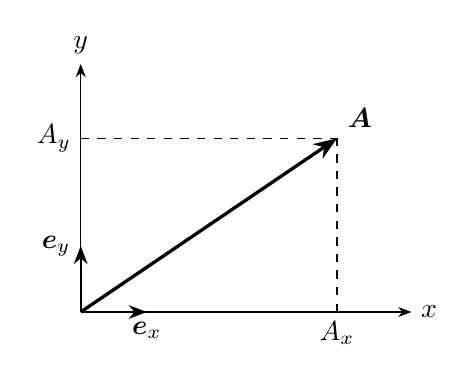
\begin{tikzpicture}[>=Stealth,scale=1.05]
    \draw[->] (0,0)--(4,0) node[right] {$x$};
    \draw[->] (0,0)--(0,3) node[above] {$y$};
    \draw[->,very thick] (0,0)--(3.1,2.1) node[above right] {$\vect{A}$};
    \draw[dashed] (3.1,0) node[below] {$A_x$}--(3.1,2.1);
    \draw[dashed] (0,2.1) node[left] {$A_y$}--(3.1,2.1);
    \draw[->,thick] (0,0)--(0.8,0) node[below] {$\unit{x}$};
    \draw[->,thick] (0,0)--(0,0.8) node[left] {$\unit{y}$};
  \end{tikzpicture}
  \caption{正規直交基底によるベクトルの成分表示}
\end{figure}

\subsubsection{スカラー場とベクトル場}

空間の各点 $P$ に一つの数 $\phi(P)$ を対応させたものを
\textbf{スカラー場}という。温度や密度がその例である。
スカラー場の変化率は勾配
\begin{equation}
  \nabla\phi=
  \frac{\partial\phi}{\partial x}\unit{x}
  +\frac{\partial\phi}{\partial y}\unit{y}
  +\frac{\partial\phi}{\partial z}\unit{z}
\end{equation}
で表される。勾配は、値が最も速く増加する向きを向き、その大きさは
その方向の変化率を表す。

\begin{figure}[htbp]
  \centering
  \begin{tikzpicture}[>=Stealth,scale=.95]
    \draw[rounded corners,fill=blue!4] (0,0) rectangle (5,3.1);
    \foreach \r in {.35,.65,1.0}
      \draw[blue!55] (2.4,1.6) ellipse ({\r*1.45} and {\r});
    \fill (1.45,1.15) circle (1.5pt) node[below left] {$P$};
    \node at (2.4,1.6) {$\phi$ が大きい};
    \draw[->,very thick,red!70!black] (1.45,1.15)--(2.65,1.75)
      node[above] {$\nabla\phi$};
    \node[align=left] at (7.3,2.2) {各点に数 $\phi(P)$\\$\Rightarrow$ スカラー場};
    \node[align=left] at (7.3,.8) {最大増加方向\\$\Rightarrow$ 勾配ベクトル};
  \end{tikzpicture}
  \caption{スカラー場とその勾配}
\end{figure}

\subsection{ベクトルの演算}

ベクトルの和は平行四辺形の対角線として幾何学的に表される。
成分表示では、対応する成分どうしを加えればよい。
\begin{equation}
  \vect{A}+\vect{B}
  =\begin{pmatrix}A_x+B_x\\A_y+B_y\\A_z+B_z\end{pmatrix}.
\end{equation}

\begin{figure}[htbp]
  \centering
  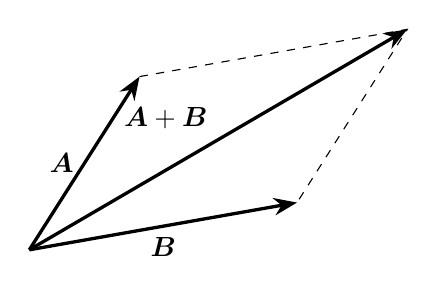
\begin{tikzpicture}[>=Stealth]
    \coordinate (O) at (0,0); \coordinate (A) at (1.4,2.2);
    \coordinate (B) at (3.4,.6); \coordinate (C) at ($(A)+(B)$);
    \draw[->,very thick] (O)--(A) node[midway,left] {$\vect{A}$};
    \draw[->,very thick] (O)--(B) node[midway,below] {$\vect{B}$};
    \draw[dashed] (A)--(C)--(B);
    \draw[->,very thick] (O)--(C) node[midway,above left] {$\vect{A}+\vect{B}$};
  \end{tikzpicture}
  \caption{ベクトルの加法（平行四辺形則）}
\end{figure}

加法とスカラー倍には、次の法則が成り立つ。
\begin{align}
  \vect{A}+\vect{B}&=\vect{B}+\vect{A}, &
  \vect{A}+(\vect{B}+\vect{C})&=(\vect{A}+\vect{B})+\vect{C},\\
  (ab)\vect{A}&=a(b\vect{A}), &
  (a+b)\vect{A}&=a\vect{A}+b\vect{A},\\
  a(\vect{A}+\vect{B})&=a\vect{A}+a\vect{B}.&&
\end{align}

\begin{example}[内分点の位置ベクトル]
位置ベクトル $\vect{r}_1,\vect{r}_2$ の点を結ぶ線分を
$m_2:m_1$ に内分する点の位置ベクトルは
\begin{equation}
  \vect{R}=\vect{r}_1+\frac{m_2}{m_1+m_2}(\vect{r}_2-\vect{r}_1)
  =\frac{m_1\vect{r}_1+m_2\vect{r}_2}{m_1+m_2}
\end{equation}
である。
\begin{center}
  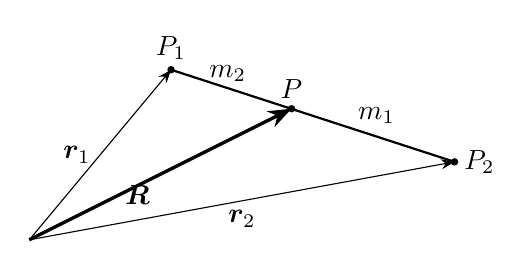
\begin{tikzpicture}[>=Stealth,scale=.9]
    \coordinate (O) at (0,0); \coordinate (P1) at (2,2.4);
    \coordinate (P2) at (6,1.1); \coordinate (P) at (3.7,1.85);
    \draw[->] (O)--(P1) node[midway,left] {$\vect{r}_1$};
    \draw[->] (O)--(P2) node[midway,below] {$\vect{r}_2$};
    \draw[->,very thick] (O)--(P) node[midway,below left] {$\vect{R}$};
    \draw[thick] (P1)--(P2);
    \fill (P1) circle (1.5pt) node[above] {$P_1$};
    \fill (P) circle (1.5pt) node[above] {$P$};
    \fill (P2) circle (1.5pt) node[right] {$P_2$};
    \node at (2.8,2.35) {$m_2$}; \node at (4.9,1.75) {$m_1$};
  \end{tikzpicture}
\end{center}
\end{example}

\subsection{内積（スカラー積）}

\begin{definition}
二つのベクトル $\vect{A},\vect{B}$ のなす角を $\theta$ とするとき、
\begin{equation}
  \vect{A}\cdot\vect{B}=|\vect{A}|\,|\vect{B}|\cos\theta
\end{equation}
を両者の\textbf{内積}という。内積の結果はスカラーである。
\end{definition}

特に $\vect{A}=\vect{B}$ とすれば
\begin{equation}
  \vect{A}\cdot\vect{A}=|\vect{A}|^2,\qquad
  |\vect{A}|=\sqrt{\vect{A}\cdot\vect{A}}
\end{equation}
である。正規直交基底を用いると
\begin{equation}
  \vect{A}\cdot\vect{B}=A_xB_x+A_yB_y+A_zB_z,\qquad
  |\vect{A}|=\sqrt{A_x^2+A_y^2+A_z^2}
\end{equation}
となる。

この成分公式は、基底の直交性から直接導ける。実際、
\begin{align}
 \vect{A}\cdot\vect{B}
 &= (A_x\unit{x}+A_y\unit{y}+A_z\unit{z})
    \cdot(B_x\unit{x}+B_y\unit{y}+B_z\unit{z}) \notag\\
 &=A_xB_x(\unit{x}\cdot\unit{x})
   +A_yB_y(\unit{y}\cdot\unit{y})
   +A_zB_z(\unit{z}\cdot\unit{z}) \notag\\
 &=A_xB_x+A_yB_y+A_zB_z.
\end{align}
異なる基底ベクトルどうしの内積は $0$ なので、交差項はすべて消える。

\begin{figure}[htbp]
  \centering
  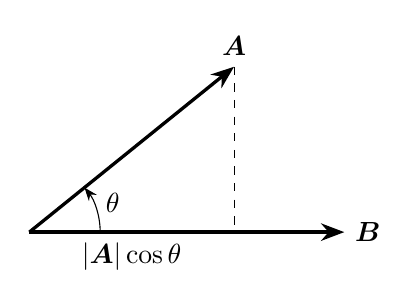
\begin{tikzpicture}[>=Stealth]
    \coordinate (O) at (0,0); \coordinate (B) at (4,0); \coordinate (A) at (2.6,2.1);
    \draw[->,very thick] (O)--(B) node[right] {$\vect{B}$};
    \draw[->,very thick] (O)--(A) node[above] {$\vect{A}$};
    \draw[dashed] (A)--(2.6,0);
    \draw[very thick] (O)--(2.6,0) node[midway,below] {$|\vect{A}|\cos\theta$};
    \pic[draw,->,"$\theta$",angle radius=9mm,angle eccentricity=1.25]
      {angle=B--O--A};
  \end{tikzpicture}
  \caption{$\vect{A}$ の $\vect{B}$ 方向への射影}
\end{figure}

内積は交換法則と分配法則を満たす。
\begin{align}
  \vect{A}\cdot\vect{B}&=\vect{B}\cdot\vect{A},\\
  \vect{A}\cdot(\vect{B}+\vect{C})
  &=\vect{A}\cdot\vect{B}+\vect{A}\cdot\vect{C},\\
  a(\vect{A}\cdot\vect{B})&=(a\vect{A})\cdot\vect{B}
  =\vect{A}\cdot(a\vect{B}).
\end{align}

\begin{example}
$P_1=(1,1),P_2=(5,1),P_3=(5,3)$ とする。
$\vect{A}=\overrightarrow{P_1P_3}=(4,2)^{\mathsf T}$、
$\vect{B}=\overrightarrow{P_1P_2}=(4,0)^{\mathsf T}$ なので
\begin{equation}
 \cos\theta=\frac{\vect{A}\cdot\vect{B}}{|\vect{A}|\,|\vect{B}|}
 =\frac{16}{\sqrt{20}\cdot4}=\frac{2}{\sqrt5}.
\end{equation}
\begin{center}
  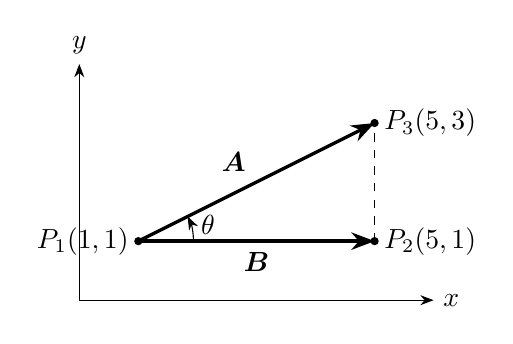
\begin{tikzpicture}[>=Stealth,scale=.75]
    \draw[->] (0,0)--(6,0) node[right] {$x$};
    \draw[->] (0,0)--(0,4) node[above] {$y$};
    \coordinate (P1) at (1,1); \coordinate (P2) at (5,1);
    \coordinate (P3) at (5,3);
    \draw[->,very thick] (P1)--(P2) node[midway,below] {$\vect{B}$};
    \draw[->,very thick] (P1)--(P3) node[midway,above left] {$\vect{A}$};
    \draw[dashed] (P2)--(P3);
    \fill (P1) circle (2pt) node[left] {$P_1(1,1)$};
    \fill (P2) circle (2pt) node[right] {$P_2(5,1)$};
    \fill (P3) circle (2pt) node[right] {$P_3(5,3)$};
    \pic[draw,->,"$\theta$",angle radius=7mm,angle eccentricity=1.3]
      {angle=P2--P1--P3};
  \end{tikzpicture}
\end{center}
\end{example}

\subsection{外積（ベクトル積）}

\begin{definition}
三次元ベクトル $\vect{A},\vect{B}$ に対して、
\begin{equation}
  \vect{A}\times\vect{B}
  =|\vect{A}|\,|\vect{B}|\sin\theta\,\vect{n}
\end{equation}
を\textbf{外積}という。$\vect{n}$ は $\vect{A},\vect{B}$ の張る面に
垂直な単位ベクトルで、その向きは右ねじの規則で定める。
\end{definition}

$|\vect{A}\times\vect{B}|$ は二つのベクトルが張る平行四辺形の面積に等しい。

\begin{figure}[htbp]
  \centering
  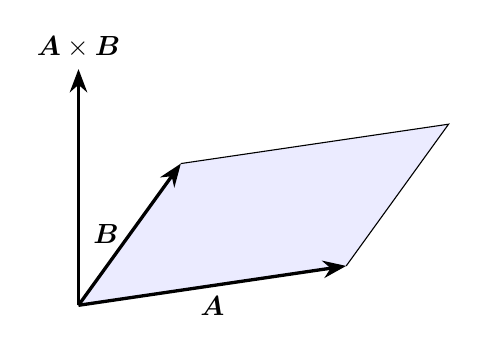
\begin{tikzpicture}[>=Stealth]
    \coordinate (O) at (0,0); \coordinate (A) at (3.4,.5);
    \coordinate (B) at (1.3,1.8); \coordinate (C) at ($(A)+(B)$);
    \fill[blue!8] (O)--(A)--(C)--(B)--cycle;
    \draw[->,very thick] (O)--(A) node[midway,below] {$\vect{A}$};
    \draw[->,very thick] (O)--(B) node[midway,left] {$\vect{B}$};
    \draw (A)--(C)--(B);
    \draw[->,very thick] (O)--(0,3) node[above] {$\vect{A}\times\vect{B}$};
  \end{tikzpicture}
  \caption{外積の向きと平行四辺形の面積}
\end{figure}

外積には次の性質がある。
\begin{align}
  \vect{A}\times\vect{B}&=-\vect{B}\times\vect{A},\\
  \vect{A}\times(\vect{B}+\vect{C})
  &=\vect{A}\times\vect{B}+\vect{A}\times\vect{C},\\
  a(\vect{A}\times\vect{B})&=(a\vect{A})\times\vect{B}
  =\vect{A}\times(a\vect{B}).
\end{align}
正規直交基底では
\begin{equation}
 \unit{x}\times\unit{y}=\unit{z},\quad
 \unit{y}\times\unit{z}=\unit{x},\quad
 \unit{z}\times\unit{x}=\unit{y}
\end{equation}
であり、同じ基底ベクトルどうしの外積は零ベクトルである。したがって
\begin{equation}
 \vect{A}\times\vect{B}=
 \begin{vmatrix}
   \unit{x}&\unit{y}&\unit{z}\\
   A_x&A_y&A_z\\
   B_x&B_y&B_z
 \end{vmatrix}
 =\begin{pmatrix}
 A_yB_z-A_zB_y\\A_zB_x-A_xB_z\\A_xB_y-A_yB_x
 \end{pmatrix}.
\end{equation}

上の行列式を展開すると、各成分がどこから現れるかを確認できる。
\begin{align}
 \vect{A}\times\vect{B}
 ={}&(A_yB_z-A_zB_y)\unit{x}
 +(A_zB_x-A_xB_z)\unit{y} \notag\\
 &+(A_xB_y-A_yB_x)\unit{z}.
\end{align}
外積は順序を入れ替えると符号が反転するため、内積とは異なり交換法則を
満たさない点に注意する。

\begin{example}
$\vect{A}=(1,-1,2)^{\mathsf T}$、$\vect{B}=(3,1,-1)^{\mathsf T}$ のとき
\begin{equation}
 \vect{A}\times\vect{B}
 =\begin{pmatrix}(-1)(-1)-2\cdot1\\2\cdot3-1(-1)\\1\cdot1-(-1)3\end{pmatrix}
 =\begin{pmatrix}-1\\7\\4\end{pmatrix}.
\end{equation}
\end{example}

\subsection{外積による多角形の面積}

$xy$ 平面上の頂点 $P_k=(x_k,y_k,0)^{\mathsf T}$
（$k=1,\ldots,N$）を反時計回りに並べ、$P_{N+1}=P_1$ とする。
原点と隣り合う二頂点が作る符号付き三角形の面積を足すと
\begin{equation}
 S=\frac12\sum_{k=1}^{N}(\vect{P}_k\times\vect{P}_{k+1})_z
  =\frac12\sum_{k=1}^{N}(x_ky_{k+1}-x_{k+1}y_k)
\end{equation}
を得る。頂点が時計回りなら右辺は負になるため、一般には絶対値を取る。
凹多角形でも、外側へ張り出した三角形と切り欠き側の三角形が逆符号に
なるので、同じ公式をそのまま利用できる。

\begin{figure}[htbp]
  \centering
  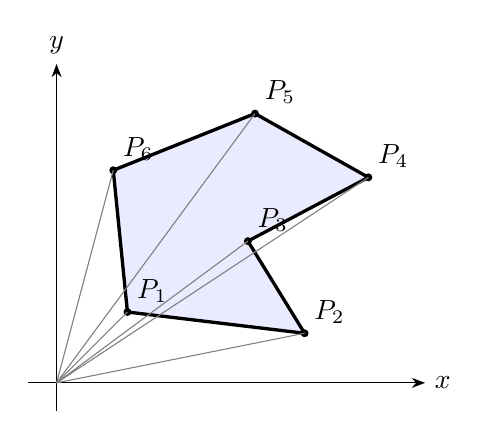
\begin{tikzpicture}[>=Stealth,scale=.9]
    \draw[->] (-.4,0)--(5.2,0) node[right] {$x$};
    \draw[->] (0,-.4)--(0,4.5) node[above] {$y$};
    \coordinate (P1) at (1,1); \coordinate (P2) at (3.5,.7);
    \coordinate (P3) at (2.7,2.0); \coordinate (P4) at (4.4,2.9);
    \coordinate (P5) at (2.8,3.8); \coordinate (P6) at (.8,3);
    \fill[blue!8] (P1)--(P2)--(P3)--(P4)--(P5)--(P6)--cycle;
    \draw[very thick] (P1)--(P2)--(P3)--(P4)--(P5)--(P6)--cycle;
    \foreach \p/\name in {P1/P_1,P2/P_2,P3/P_3,P4/P_4,P5/P_5,P6/P_6}
      {\fill (\p) circle (1.6pt) node[above right] {$\name$};\draw[gray] (0,0)--(\p);}
  \end{tikzpicture}
  \caption{三角形への分割による多角形の符号付き面積}
\end{figure}

\begin{example}
$P_1=(1,2),P_2=(5,2),P_3=(5,4)$ の三角形では
\begin{equation}
 S=\frac12\{(1\cdot2-5\cdot2)+(5\cdot4-5\cdot2)
 +(5\cdot2-1\cdot4)\}=4.
\end{equation}
\end{example}

\subsection{行列}

\subsubsection{行列の成分と基本演算}

$m$ 行 $n$ 列の数の配列
\begin{equation}
 A=(a_{ij})=
 \begin{pmatrix}
  a_{11}&a_{12}&\cdots&a_{1n}\\
  a_{21}&a_{22}&\cdots&a_{2n}\\
  \vdots&\vdots&\ddots&\vdots\\
  a_{m1}&a_{m2}&\cdots&a_{mn}
 \end{pmatrix}
\end{equation}
を $m\times n$ 行列という。$a_{ij}$ の第1添字 $i$ は行、第2添字
$j$ は列を表す。

\begin{figure}[htbp]
\centering
\begin{tikzpicture}[>=Stealth]
 \matrix (A) [matrix of math nodes,left delimiter=(,right delimiter=),
  row sep=7mm,column sep=10mm,nodes={minimum width=9mm}] {
  a_{11}&a_{12}&a_{13}\\ a_{21}&a_{22}&a_{23}\\};
 \node[draw=blue,rounded corners,fit=(A-1-1)(A-1-3),inner sep=3pt] (row) {};
 \node[draw=red,rounded corners,fit=(A-1-1)(A-2-1),inner sep=3pt] (col) {};
 \draw[->,blue] ($(row.east)+(8mm,5mm)$)--(row.east)
   node[pos=0,above] {第1行};
 \draw[->,red] ($(col.south)+(-8mm,-7mm)$)--(col.south)
   node[pos=0,below] {第1列};
\end{tikzpicture}
\caption{行と列、および成分の添字}
\end{figure}

同じ型の行列どうしの和・差は成分ごとに計算する。たとえば
\begin{equation}
 \begin{pmatrix}1&-1&3\\4&-2&-1\end{pmatrix}
 +\begin{pmatrix}3&-1&1\\2&3&6\end{pmatrix}
 =\begin{pmatrix}4&-2&4\\6&1&5\end{pmatrix}.
\end{equation}
また、スカラー $k$ との積は全成分を $k$ 倍して
\[
 kA=(ka_{ij}),\qquad
 2\begin{pmatrix}2&3\\-1&4\end{pmatrix}
 =\begin{pmatrix}4&6\\-2&8\end{pmatrix}
\]
とする。

\subsubsection{行列の積}

$A$ が $m\times n$ 行列、$B$ が $n\times p$ 行列なら、積 $AB$ は
$m\times p$ 行列であり
\begin{equation}
 (AB)_{ij}=\sum_{k=1}^{n}a_{ik}b_{kj}
\end{equation}
と定義する。すなわち、$A$ の第 $i$ 行と $B$ の第 $j$ 列を
成分ごとに掛け、その和を取る。

\begin{figure}[htbp]
\centering
\begin{tikzpicture}[>=Stealth,every node/.style={font=\small}]
 \matrix (A) [matrix of math nodes,left delimiter=(,right delimiter=),
   row sep=5mm,column sep=7mm] {
  1&-1&3\\4&-2&-1\\};
 \node at ($(A.east)+(5mm,0)$) {$\times$};
 \matrix (B) [matrix of math nodes,right=13mm of A,
   left delimiter=(,right delimiter=),row sep=5mm,column sep=7mm] {
  3&2\\-1&3\\1&6\\};
 \node at ($(B.east)+(5mm,0)$) {$=$};
 \matrix (C) [matrix of math nodes,right=13mm of B,
   left delimiter=(,right delimiter=),row sep=5mm,column sep=9mm] {
  |[draw=purple,fill=purple!8]|7&17\\13&-4\\};
 \node[draw=blue,rounded corners,fit=(A-1-1)(A-1-3),inner sep=2pt] {};
 \node[draw=red,rounded corners,fit=(B-1-1)(B-3-1),inner sep=2pt] {};
 \draw[->,blue,bend left=18] (A-1-2.north)--(C-1-1.north)
   node[midway,above] {行};
 \draw[->,red,bend right=18] (B-2-1.south)--(C-1-1.south)
   node[midway,below] {列};
\end{tikzpicture}
\[
 \underbrace{1\cdot3+(-1)(-1)+3\cdot1}_{第1行と第1列}=7
\]
\caption{行列積の計算：行と列の内積が一つの成分になる}
\end{figure}

行列をベクトルに掛ける操作も同じ規則であり、線形変換を表す。
\[
 \vect{v}'=A\vect{v}
 =\begin{pmatrix}2&3\\-1&4\end{pmatrix}
  \begin{pmatrix}-1\\3\end{pmatrix}
 =\begin{pmatrix}7\\13\end{pmatrix}.
\]

行列積には
\begin{align}
 (kA)B&=k(AB)=A(kB),&
 A(BC)&=(AB)C,\\
 (A+B)C&=AC+BC,&
 C(A+B)&=CA+CB
\end{align}
が成り立つ。ただし一般には $AB\ne BA$ であり、交換法則は成り立たない。

\subsubsection{単位行列}

対角成分がすべて $1$、それ以外が $0$ の正方行列を単位行列という。
\[
 I_n=\begin{pmatrix}
 1&0&\cdots&0\\0&1&\ddots&\vdots\\
 \vdots&\ddots&\ddots&0\\0&\cdots&0&1
 \end{pmatrix},\qquad
 AI_n=I_nA=A,\qquad I_n^k=I_n.
\]
単位行列は、数の掛け算における $1$ と同じ役割をもつ。

\subsection{行列式}

\subsubsection{2次・3次の行列式}

正方行列 $A$ の行列式を $\det A$ または $|A|$ と書く。2次では
\begin{equation}
 \begin{vmatrix}a_{11}&a_{12}\\a_{21}&a_{22}\end{vmatrix}
 =a_{11}a_{22}-a_{12}a_{21}.
\end{equation}

\begin{figure}[htbp]
\centering
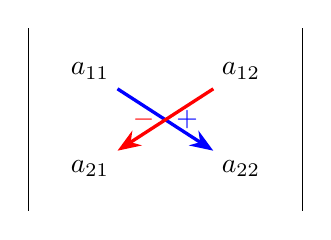
\begin{tikzpicture}[>=Stealth]
 \matrix (M) [matrix of math nodes,row sep=8mm,column sep=12mm] {
  a_{11}&a_{12}\\a_{21}&a_{22}\\};
 \draw[->,very thick,blue] (M-1-1)--(M-2-2)
   node[midway,right] {$+$};
 \draw[->,very thick,red] (M-1-2)--(M-2-1)
   node[midway,left] {$-$};
 \draw ($(M.north west)+(-3mm,2mm)$)--($(M.south west)+(-3mm,-2mm)$);
 \draw ($(M.north east)+(3mm,2mm)$)--($(M.south east)+(3mm,-2mm)$);
\end{tikzpicture}
\caption{2次行列式：右下がりを加え、左下がりを引く}
\end{figure}

3次では最初の2列を右側へ写して斜めの積を取る
\textbf{サラスの方法}が使える。
\begin{align}
 \det A={}&a_{11}a_{22}a_{33}+a_{12}a_{23}a_{31}
 +a_{13}a_{21}a_{32}\notag\\
 &-a_{13}a_{22}a_{31}-a_{11}a_{23}a_{32}
 -a_{12}a_{21}a_{33}.
\end{align}

\begin{figure}[htbp]
\centering
\begin{tikzpicture}[x=1.5cm,y=1cm,>=Stealth]
 % 元の3列
 \node (m11) at (1,-1) {$a_{11}$};
 \node (m12) at (2,-1) {$a_{12}$};
 \node (m13) at (3,-1) {$a_{13}$};
 \node (m21) at (1,-2) {$a_{21}$};
 \node (m22) at (2,-2) {$a_{22}$};
 \node (m23) at (3,-2) {$a_{23}$};
 \node (m31) at (1,-3) {$a_{31}$};
 \node (m32) at (2,-3) {$a_{32}$};
 \node (m33) at (3,-3) {$a_{33}$};
 % 右側へ複写した最初の2列
 \node[blue!65!black] (m14) at (4,-1) {$a_{11}$};
 \node[blue!65!black] (m15) at (5,-1) {$a_{12}$};
 \node[blue!65!black] (m24) at (4,-2) {$a_{21}$};
 \node[blue!65!black] (m25) at (5,-2) {$a_{22}$};
 \node[blue!65!black] (m34) at (4,-3) {$a_{31}$};
 \node[blue!65!black] (m35) at (5,-3) {$a_{32}$};
 \draw[thick] (.55,-.55)--(.55,-3.45);
 \draw[thick] (3.45,-.55)--(3.45,-3.45);
 \draw[dashed,blue!65!black] (3.5,-.55)--(3.5,-3.45);
 % 正の3項（右下がり）
 \draw[blue,->,very thick,opacity=.75] ($(m11)+(-.25,.25)$)--($(m22)+(0,.25)$)--($(m33)+(.25,.25)$);
 \draw[blue,->,very thick,opacity=.75] ($(m12)+(-.25,.25)$)--($(m23)+(0,.25)$)--($(m34)+(.25,.25)$);
 \draw[blue,->,very thick,opacity=.75] ($(m13)+(-.25,.25)$)--($(m24)+(0,.25)$)--($(m35)+(.25,.25)$);
 % 負の3項（右上がり）
 \draw[red,->,very thick,opacity=.75] ($(m31)+(-.25,-.25)$)--($(m22)+(0,-.25)$)--($(m13)+(.25,-.25)$);
 \draw[red,->,very thick,opacity=.75] ($(m32)+(-.25,-.25)$)--($(m23)+(0,-.25)$)--($(m14)+(.25,-.25)$);
 \draw[red,->,very thick,opacity=.75] ($(m33)+(-.25,-.25)$)--($(m24)+(0,-.25)$)--($(m15)+(.25,-.25)$);
 \node[blue,anchor=west] at (5.65,-1.35) {$+$：右下がり3項};
 \node[red,anchor=west] at (5.65,-2.65) {$-$：右上がり3項};
 \draw[decorate,decoration={brace,mirror,amplitude=5pt},blue!65!black]
   (3.65,-3.5)--(5.35,-3.5)
   node[midway,below=6pt] {最初の2列を複写};
\end{tikzpicture}
\caption{サラスの方法（3次行列式にのみ使用できる）}
\end{figure}

\subsubsection{小行列式・余因子と展開}

$a_{ij}$ のある第 $i$ 行と第 $j$ 列を除いてできる行列の行列式を
小行列式 $M_{ij}$、符号を付けた
\begin{equation}
 C_{ij}=(-1)^{i+j}M_{ij}
\end{equation}
を余因子という。任意の一つの行または列に沿って
\begin{equation}
 \det A=\sum_{j=1}^{n}a_{ij}C_{ij}
       =\sum_{j=1}^{n}(-1)^{i+j}a_{ij}M_{ij}
\end{equation}
と展開できる。どの行・列を選んでも答えは同じである。

\begin{figure}[htbp]
\centering
\begin{tikzpicture}
 \matrix (A) [matrix of math nodes,left delimiter=(,right delimiter=),
  row sep=7mm,column sep=9mm,nodes={minimum width=8mm}] {
  a_{11}&a_{12}&a_{13}\\a_{21}&a_{22}&a_{23}\\a_{31}&a_{32}&a_{33}\\};
 \node[fill=red!14,fit=(A-2-1)(A-2-3),inner sep=1pt] {};
 \node[fill=red!14,fit=(A-1-2)(A-3-2),inner sep=1pt] {};
 \node[draw=blue,very thick,fit=(A-1-1)(A-1-3)(A-3-1)(A-3-3),
   inner sep=2pt,label=right:{$M_{22}$ に残る4成分}] {};
 \node[draw,circle,inner sep=2pt] at (A-2-2) {$a_{22}$};
\end{tikzpicture}
\caption{$M_{22}$：$a_{22}$ の行と列を除く}
\end{figure}

第1行で展開する3次の公式は
\begin{align}
 \det A={}&a_{11}\begin{vmatrix}a_{22}&a_{23}\\a_{32}&a_{33}\end{vmatrix}
 -a_{12}\begin{vmatrix}a_{21}&a_{23}\\a_{31}&a_{33}\end{vmatrix}\notag\\
 &+a_{13}\begin{vmatrix}a_{21}&a_{22}\\a_{31}&a_{32}\end{vmatrix}.
\end{align}

\subsubsection{行列式の性質}

計算では次の性質が重要である。
\begin{enumerate}
 \item \textbf{どの行（または列）で余因子展開しても値は同じ。}

 \item \textbf{転置しても値は変わらない。}

  行と列を入れ替えた転置行列
  \[
   A=\begin{pmatrix}a_{11}&a_{12}\\a_{21}&a_{22}\end{pmatrix},
   \qquad
   A^{\mathsf T}=\begin{pmatrix}a_{11}&a_{21}\\a_{12}&a_{22}\end{pmatrix}
  \]
  について
  \[
   \det A=a_{11}a_{22}-a_{12}a_{21}
   =\det A^{\mathsf T}
  \]
  である。

 \item \textbf{一つの行（列）がすべて $0$ なら行列式は $0$。}

  零の行に沿って余因子展開すると各項がすべて $0$ になる。たとえば
  \[
   \begin{vmatrix}
    a_{11}&a_{12}&a_{13}\\
    0&0&0\\
    a_{31}&a_{32}&a_{33}
   \end{vmatrix}=0.
  \]

 \item \textbf{二つの行（列）を交換すると符号が反転する。}

  たとえば
  \[
   \begin{vmatrix}3&1\\-1&2\end{vmatrix}=7,\qquad
   \begin{vmatrix}-1&2\\3&1\end{vmatrix}=-7.
  \]
  第1行と第2行を交換したため、絶対値は同じで符号だけが変わる。

 \item \textbf{一つの行（列）を $k$ 倍すると行列式も $k$ 倍される。}

  \[
   \begin{vmatrix}3&1\\-k&2k\end{vmatrix}
   =k\begin{vmatrix}3&1\\-1&2\end{vmatrix}=7k.
  \]
  第2行から共通因子 $k$ を行列式の外へ出した形である。

 \item \textbf{二つの行（列）が比例すれば行列式は $0$。}

  \[
   \begin{vmatrix}3&1\\6&2\end{vmatrix}
   =3\cdot2-1\cdot6=0.
  \]
  第2行は第1行の2倍なので、二つの行が同じ方向の情報しかもたない。

 \item \textbf{ある行の定数倍を別の行に加えても値は変わらない。}

  例として
  \[
   D=\begin{vmatrix}2&1&5\\3&-2&4\\8&1&7\end{vmatrix}
  \]
  で、$R_2\leftarrow R_2+2R_1$ および
  $R_3\leftarrow R_3-R_1$ としても
  \[
   D=\begin{vmatrix}2&1&5\\7&0&14\\6&0&2\end{vmatrix}=70
  \]
  と値は変わらない。詳しい操作図を次に示す。
\end{enumerate}

\begin{example}[性質7：余因子展開と行操作]
\[
D=\begin{vmatrix}2&1&5\\3&-2&4\\8&1&7\end{vmatrix}.
\]
第1行で展開すると
\[
D=2(-14-4)-(21-32)+5(3+16)=70.
\]
同じ計算を行操作で行うと、次の注釈図のようになる。
\begin{center}
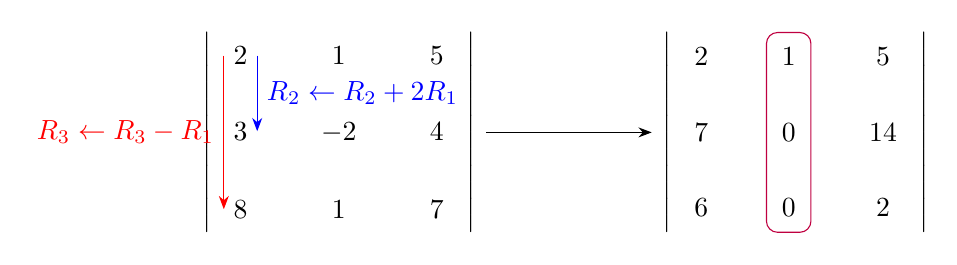
\begin{tikzpicture}[>=Stealth]
 \matrix (A) [matrix of math nodes,left delimiter=|,right delimiter=|,
  row sep=5mm,column sep=7mm] {2&1&5\\3&-2&4\\8&1&7\\};
 \matrix (B) [matrix of math nodes,right=27mm of A,left delimiter=|,
  right delimiter=|,row sep=5mm,column sep=7mm] {2&1&5\\7&0&14\\6&0&2\\};
 \draw[->] ($(A.east)+(3mm,0)$)--($(B.west)+(-3mm,0)$);
 \draw[->,blue,bend left=20] (A-1-1.east)--(A-2-1.east)
   node[midway,right] {$R_2\leftarrow R_2+2R_1$};
 \draw[->,red,bend right=25] (A-1-1.west)--(A-3-1.west)
   node[midway,left] {$R_3\leftarrow R_3-R_1$};
 \node[draw=purple,rounded corners,fit=(B-1-2)(B-3-2),inner sep=2pt] {};
\end{tikzpicture}
\[
D=-\begin{vmatrix}7&14\\6&2\end{vmatrix}
=-(14-84)=70.
\]
\end{center}
第2列に零を作ったので、その列で余因子展開すれば一つの項だけで済む。
\end{example}

\subsubsection{上三角化による計算}

上三角行列では対角成分の積が行列式になる：
\[
\det\begin{pmatrix}
a_{11}&*&\cdots&*\\0&a_{22}&\cdots&*\\
\vdots&\ddots&\ddots&\vdots\\0&\cdots&0&a_{nn}
\end{pmatrix}
=\prod_{k=1}^{n}a_{kk}.
\]
したがって、行列式を変えない「他の行の定数倍を加える」操作で
対角線より下を $0$ にすればよい。

\begin{example}
\begin{align}
\begin{vmatrix}1&-1&2\\1&2&3\\0&1&2\end{vmatrix}
&\xrightarrow{R_2\leftarrow R_2-R_1}
\begin{vmatrix}1&-1&2\\0&3&1\\0&1&2\end{vmatrix}\notag\\
&\xrightarrow{R_3\leftarrow R_3-\frac13R_2}
\begin{vmatrix}1&-1&2\\0&3&1\\0&0&\frac53\end{vmatrix}
=1\cdot3\cdot\frac53=5.
\end{align}
\end{example}

\subsection{逆行列}

\subsubsection{定義と公式}

$AA^{-1}=A^{-1}A=I$ を満たす $A^{-1}$ を $A$ の逆行列という。
逆行列が存在するための必要十分条件は $\det A\ne0$ である。2次では
\begin{equation}
A^{-1}=\frac1{\det A}
\begin{pmatrix}a_{22}&-a_{12}\\-a_{21}&a_{11}\end{pmatrix},
\qquad
\det A=a_{11}a_{22}-a_{12}a_{21}.
\end{equation}
つまり、対角成分を交換し、非対角成分の符号を反転して行列式で割る。

一般の $n$ 次正方行列では、余因子行列を転置した随伴行列を使って
\begin{equation}
A^{-1}=\frac1{\det A}\operatorname{adj}A
=\frac1{\det A}
\begin{pmatrix}
C_{11}&C_{21}&\cdots&C_{n1}\\
C_{12}&C_{22}&\cdots&C_{n2}\\
\vdots&\vdots&\ddots&\vdots\\
C_{1n}&C_{2n}&\cdots&C_{nn}
\end{pmatrix}.
\end{equation}
余因子の行と列が入れ替わっていることに注意する。

\subsection{連立一次方程式}

\subsubsection{行列による表現}

$n$ 個の未知数をもつ $n$ 本の連立一次方程式は
\begin{equation}
 \begin{cases}
  a_{11}x_1+\cdots+a_{1n}x_n=b_1,\\
  \hfill\vdots\\
  a_{n1}x_1+\cdots+a_{nn}x_n=b_n
 \end{cases}
 \quad\Longleftrightarrow\quad
 A\vect{x}=\vect{b}
\end{equation}
と書ける。ここで $A=(a_{ij})$ は\textbf{係数行列}、
$\vect{x}=(x_1,\ldots,x_n)^{\mathsf T}$ は未知数ベクトル、
$\vect{b}=(b_1,\ldots,b_n)^{\mathsf T}$ は定数ベクトルである。
$\det A\ne0$ なら逆行列が存在し、
\begin{equation}
 \boxed{\vect{x}=A^{-1}\vect{b}}
\end{equation}
となる。ただし、実際の数値計算では以下のクラメルの公式や
掃き出し法を使う方が計算の見通しがよいことが多い。

\subsubsection{クラメルの公式}

まず2元連立一次方程式
\begin{equation}
 \begin{cases}
  a_{11}x_1+a_{12}x_2=b_1, &(1)\\
  a_{21}x_1+a_{22}x_2=b_2. &(2)
 \end{cases}
\end{equation}
を加減法で解く。$a_{22}\times(1)-a_{12}\times(2)$ と
$a_{11}\times(2)-a_{21}\times(1)$ を作ると、
\begin{align}
 (a_{11}a_{22}-a_{12}a_{21})x_1&=b_1a_{22}-a_{12}b_2,\label{eq:cramer-x1}\\
 (a_{11}a_{22}-a_{12}a_{21})x_2&=a_{11}b_2-b_1a_{21}.\label{eq:cramer-x2}
\end{align}
これは行列式を用いて
\begin{align}
 \begin{vmatrix}a_{11}&a_{12}\\a_{21}&a_{22}\end{vmatrix}x_1
 &=\begin{vmatrix}b_1&a_{12}\\b_2&a_{22}\end{vmatrix},&
 \begin{vmatrix}a_{11}&a_{12}\\a_{21}&a_{22}\end{vmatrix}x_2
 &=\begin{vmatrix}a_{11}&b_1\\a_{21}&b_2\end{vmatrix}
\end{align}
と表せる。そこで
\[
 D=\begin{vmatrix}a_{11}&a_{12}\\a_{21}&a_{22}\end{vmatrix},\quad
 D_1=\begin{vmatrix}b_1&a_{12}\\b_2&a_{22}\end{vmatrix},\quad
 D_2=\begin{vmatrix}a_{11}&b_1\\a_{21}&b_2\end{vmatrix}
\]
とおけば、$D\ne0$ のとき
\begin{equation}
 \boxed{x_1=\frac{D_1}{D},\qquad x_2=\frac{D_2}{D}}
\end{equation}
を得る。これを\textbf{クラメルの公式}という。

一般に $A\vect{x}=\vect{b}$ に対し、$D=\det A$ とする。
$A$ の第 $k$ 列だけを $\vect{b}$ に置き換えた行列の行列式を
$D_k$ とすれば、$D\ne0$ のとき
\begin{equation}
 \boxed{x_k=\frac{D_k}{D}\quad(k=1,2,\ldots,n)}
\end{equation}
である。未知数が少ないときには便利だが、次数が大きい場合は
多数の行列式が必要になるため、掃き出し法の方が効率的である。

\subsubsection{解の個数と幾何学的意味}

2元一次方程式の各式は $x_1x_2$ 平面上の直線を表す。
したがって、連立方程式を解くことは2直線の共通点を求めることに
等しい。

\begin{figure}[htbp]
\centering
\begin{tikzpicture}[>=Stealth,scale=.9]
 \begin{scope}
  \draw[->] (-.2,0)--(3.7,0) node[right] {$x_1$};
  \draw[->] (0,-.3)--(0,3.2) node[above] {$x_2$};
  \draw[blue,thick] (.2,2.8)--(3.3,.2);
  \draw[red,thick] (.7,-.2)--(2.8,3.1);
  \fill (1.75,1.45) circle (2pt) node[right] {$P$};
  \node at (1.8,-.8) {$D\ne0$：一意解};
 \end{scope}
 \begin{scope}[xshift=5.2cm]
  \draw[->] (-.2,0)--(3.7,0) node[right] {$x_1$};
  \draw[->] (0,-.3)--(0,3.2) node[above] {$x_2$};
  \draw[blue,thick] (.2,.5)--(3.3,2.8);
  \draw[red,thick,dashed] (.2,.5)--(3.3,2.8);
  \node at (1.8,-.8) {$D=0$：無数の解};
 \end{scope}
 \begin{scope}[xshift=10.4cm]
  \draw[->] (-.2,0)--(3.7,0) node[right] {$x_1$};
  \draw[->] (0,-.3)--(0,3.2) node[above] {$x_2$};
  \draw[blue,thick] (.2,.3)--(3.3,2.5);
  \draw[red,thick] (.2,1)--(3.3,3.2);
  \node at (1.8,-.8) {$D=0$：解なし};
 \end{scope}
\end{tikzpicture}
\caption{2元連立一次方程式の三つの解のパターン}
\end{figure}

まとめると次のようになる。
\begin{enumerate}
 \item $D\ne0$：2直線は1点で交わり、解は一意に決まる。
 \item $D=0$ で、定数項まで含めて一方の式が他方の定数倍：
       2直線は一致し、解は無数にある。
 \item $D=0$ だが、定数項まで含めると比例しない：
       2直線は平行で、解はない。
\end{enumerate}
後二者を区別するには係数行列だけでなく定数項も調べる必要がある。
一般の連立方程式では、係数行列 $A$ と拡大係数行列
$[A\mid\vect{b}]$ の階数を用いて
\[
 \operatorname{rank}A=\operatorname{rank}[A\mid\vect{b}]
\]
なら解が存在し、この共通の階数が未知数の個数と等しければ一意解、
小さければ無数の解となる。階数が異なれば解は存在しない。

\subsubsection{掃き出し法（ガウス・ジョルダン法）}

連立方程式の係数と定数項を並べた
\begin{equation}
 [A\mid\vect{b}]
\end{equation}
を\textbf{拡大係数行列}という。次の三つの基本変形は方程式の解を
変えない。
\begin{enumerate}
 \item 二つの行を入れ替える。
 \item 一つの行を $0$ でない定数倍する。
 \item 一つの行に、別の行の定数倍を加える。
\end{enumerate}
これらを使って係数部分を単位行列にする手続きを掃き出し法という。

\begin{example}[掃き出し法による連立方程式の解法]
\[
 \begin{cases}
  3x+2y+z=1,\\
  x+4y-3z=-3,\\
  2x+3y+2z=5
 \end{cases}
\]
を解く。分数を避けて計算を見やすくするため、まず第1行と第2行を
交換する。
\begin{align*}
 \left(\begin{array}{ccc|c}3&2&1&1\\1&4&-3&-3\\2&3&2&5\end{array}\right)
 &\xrightarrow{R_1\leftrightarrow R_2}
 \left(\begin{array}{ccc|c}1&4&-3&-3\\3&2&1&1\\2&3&2&5\end{array}\right)\\
 &\xrightarrow[,R_3\leftarrow R_3-2R_1,]{R_2\leftarrow R_2-3R_1}
 \left(\begin{array}{ccc|c}1&4&-3&-3\\0&-10&10&10\\0&-5&8&11\end{array}\right)\\
 &\xrightarrow{R_2\leftarrow-\frac1{10}R_2}
 \left(\begin{array}{ccc|c}1&4&-3&-3\\0&1&-1&-1\\0&-5&8&11\end{array}\right)\\
 &\xrightarrow[,R_1\leftarrow R_1-4R_2,]{R_3\leftarrow R_3+5R_2}
 \left(\begin{array}{ccc|c}1&0&1&1\\0&1&-1&-1\\0&0&3&6\end{array}\right)\\
 &\longrightarrow
 \left(\begin{array}{ccc|c}1&0&0&-1\\0&1&0&1\\0&0&1&2\end{array}\right).
\end{align*}
したがって
\[
 \boxed{x=-1,\qquad y=1,\qquad z=2}.
\]
最後に元の3式へ代入すると、計算間違いを検算できる。
\end{example}

\begin{example}[演習]
次の連立方程式を掃き出し法で解け。ただし、途中で必要なら行を
入れ替えてよい。
\[
 \begin{pmatrix}1&-2&1\\-2&4&1\\3&-5&2\end{pmatrix}
 \begin{pmatrix}x\\y\\z\end{pmatrix}
 =\begin{pmatrix}0\\1\\1\end{pmatrix}.
\]
答えは次のとおりである。
\[
 \boxed{x=\frac73,\qquad y=\frac43,\qquad z=\frac13}
\]
\end{example}

\subsubsection{掃き出し法による逆行列}

$AA^{-1}=I$ である。$A^{-1}$ の各列を未知ベクトルとみれば、これは
$A\vect{x}=\unit{1},\ldots,A\vect{x}=\unit{n}$ という $n$ 組の
連立方程式である。右辺をまとめた拡大行列に同じ行基本変形を行い、
\begin{equation}
 \left(A\mid I\right)\longrightarrow\left(I\mid A^{-1}\right)
\end{equation}
とすれば逆行列を一度に求められる。途中で左側を $I$ にできなければ、
$A$ は正則でなく逆行列は存在しない。

\begin{example}[逆行列の計算]
\[
 A=\begin{pmatrix}2&1&-2\\1&1&-1\\2&3&-1\end{pmatrix}
\]
に対し、$(A\mid I)$ を掃き出す。初めに第1行と第2行を交換すると
計算しやすい。
\begin{align*}
\left(\begin{array}{ccc|ccc}2&1&-2&1&0&0\\1&1&-1&0&1&0\\2&3&-1&0&0&1\end{array}\right)
&\xrightarrow{R_1\leftrightarrow R_2}
\left(\begin{array}{ccc|ccc}1&1&-1&0&1&0\\2&1&-2&1&0&0\\2&3&-1&0&0&1\end{array}\right)\\
&\longrightarrow
\left(\begin{array}{ccc|ccc}1&0&0&2&-5&1\\0&1&0&-1&2&0\\0&0&1&1&-4&1\end{array}\right).
\end{align*}
よって
\begin{equation}
 \boxed{A^{-1}=\begin{pmatrix}2&-5&1\\-1&2&0\\1&-4&1\end{pmatrix}}.
\end{equation}
求めた後に $AA^{-1}=I$ を計算すれば、各成分をまとめて検算できる。
\end{example}

\subsection{一次変換}

ベクトル空間 $\mathbb{R}^n$ からベクトル空間 $\mathbb{R}^n$ への写像を
考える。写像 $f\colon\mathbb{R}^n\to\mathbb{R}^n$ が次の二つの性質を
満たすとき、$f$ を\textbf{一次変換}（線形写像）という。
\begin{itemize}
 \item 加法をしてから変換しても、変換してから加法をしても同じである：
 \begin{equation}
  f(\vect{v}+\vect{w})=f(\vect{v})+f(\vect{w}).
 \end{equation}
 \item スカラー倍してから変換しても、変換してからスカラー倍しても同じである：
 \begin{equation}
  f(a\vect{v})=a f(\vect{v}).
 \end{equation}
\end{itemize}

\begin{example}
変換
\[
 A=\begin{pmatrix}1&-1\\2&1\end{pmatrix},\qquad
 \vect{v}=\begin{pmatrix}2\\1\end{pmatrix},\qquad
 \vect{w}=\begin{pmatrix}-1\\1\end{pmatrix}
\]
について、加法とスカラー倍が保たれることを確かめる。
\begin{align*}
 A(\vect{v}+\vect{w})
 &=\begin{pmatrix}1&-1\\2&1\end{pmatrix}
   \left\{\begin{pmatrix}2\\1\end{pmatrix}
   +\begin{pmatrix}-1\\1\end{pmatrix}\right\}
 =\begin{pmatrix}1&-1\\2&1\end{pmatrix}
  \begin{pmatrix}1\\2\end{pmatrix}
 =\begin{pmatrix}-1\\4\end{pmatrix},\\
 A\vect{v}+A\vect{w}
 &=\begin{pmatrix}1&-1\\2&1\end{pmatrix}\begin{pmatrix}2\\1\end{pmatrix}
  +\begin{pmatrix}1&-1\\2&1\end{pmatrix}\begin{pmatrix}-1\\1\end{pmatrix}\\
 &=\begin{pmatrix}1\\5\end{pmatrix}+\begin{pmatrix}-2\\-1\end{pmatrix}
 =\begin{pmatrix}-1\\4\end{pmatrix}.
\end{align*}
また、
\begin{align*}
 A(2\vect{v})
 &=\begin{pmatrix}1&-1\\2&1\end{pmatrix}\begin{pmatrix}4\\2\end{pmatrix}
 =\begin{pmatrix}2\\10\end{pmatrix},\\
 2A\vect{v}
 &=2\begin{pmatrix}1&-1\\2&1\end{pmatrix}\begin{pmatrix}2\\1\end{pmatrix}
 =2\begin{pmatrix}1\\5\end{pmatrix}
 =\begin{pmatrix}2\\10\end{pmatrix}.
\end{align*}
\end{example}

\subsubsection{直交変換}

内積を保存する一次変換を\textbf{直交変換}という。すなわち、
\begin{align}
 (A\vect{v})\mathbin{\boldsymbol{\cdot}}(A\vect{w})
 &=(A\vect{v})^{\mathsf T}(A\vect{w})\notag\\
 &=\vect{v}^{\mathsf T}A^{\mathsf T}A\vect{w}
 =\vect{v}^{\mathsf T}\vect{w}
\end{align}
を満たす変換である。したがって、直交変換の表現行列 $A$ は
\begin{equation}
 \boxed{A^{\mathsf T}A=I}
\end{equation}
を満たす。このような行列を\textbf{直交行列}という。

直交変換について、次が成り立つ。
\begin{itemize}
 \item 逆行列は転置行列である：$A^{-1}=A^{\mathsf T}$。
 \item 行列式は $\det A=\pm1$ である。実際、
 \[
  1=\det I=\det(A^{\mathsf T}A)
   =(\det A^{\mathsf T})(\det A)=(\det A)^2.
 \]
\end{itemize}

\begin{example}
\begin{equation}
 A=\begin{pmatrix}
 \dfrac1{\sqrt2}&-\dfrac1{\sqrt2}\\[2mm]
 \dfrac1{\sqrt2}& \dfrac1{\sqrt2}
 \end{pmatrix}
\end{equation}
とする。このとき
\[
 \det A=\frac12-\left(-\frac12\right)=1,
\]
また
\[
 A^{\mathsf T}A
 =\begin{pmatrix}
 \dfrac1{\sqrt2}&\dfrac1{\sqrt2}\\[2mm]
 -\dfrac1{\sqrt2}&\dfrac1{\sqrt2}
 \end{pmatrix}
 \begin{pmatrix}
 \dfrac1{\sqrt2}&-\dfrac1{\sqrt2}\\[2mm]
 \dfrac1{\sqrt2}&\dfrac1{\sqrt2}
 \end{pmatrix}
 =\begin{pmatrix}1&0\\0&1\end{pmatrix}
\]
であるから、$A$ は直交変換である。

さらに
\[
 \vect{v}=\begin{pmatrix}2\\1\end{pmatrix},\qquad
 \vect{w}=\begin{pmatrix}-1\\1\end{pmatrix}
\]
とすると、
\[
 \vect{v}\mathbin{\boldsymbol{\cdot}}\vect{w}
 =\vect{v}^{\mathsf T}\vect{w}=-1,
\]
一方、
\[
 A\vect{v}=\begin{pmatrix}1/\sqrt2\\3/\sqrt2\end{pmatrix},\qquad
 A\vect{w}=\begin{pmatrix}-2/\sqrt2\\0\end{pmatrix}
\]
なので、
\[
 (A\vect{v})\mathbin{\boldsymbol{\cdot}}(A\vect{w})=-1
\]
となり、内積が保存されている。
\end{example}

この $A$ はどのような変換であろうか。標準基底の像は
\[
 \unit{x}'=A\unit{x}
 =\begin{pmatrix}1/\sqrt2\\1/\sqrt2\end{pmatrix},\qquad
 \unit{y}'=A\unit{y}
 =\begin{pmatrix}-1/\sqrt2\\1/\sqrt2\end{pmatrix}
\]
である。

\begin{figure}[htbp]
\centering
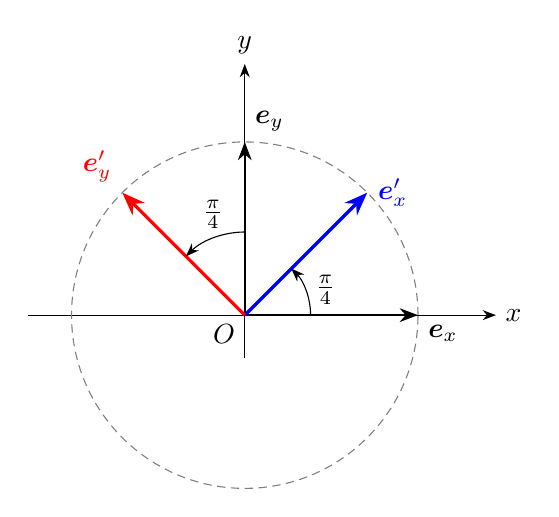
\begin{tikzpicture}[>=Stealth,scale=2.2]
 \draw[->] (-1.25,0)--(1.45,0) node[right] {$x$};
 \draw[->] (0,-.25)--(0,1.45) node[above] {$y$};
 \draw[densely dashed,gray] (0,0) circle (1);
 \draw[->,thick] (0,0)--(1,0) node[below right] {$\unit{x}$};
 \draw[->,thick] (0,0)--(0,1) node[above right] {$\unit{y}$};
 \draw[->,very thick,blue] (0,0)--({sqrt(2)/2},{sqrt(2)/2})
   node[right] {$\unit{x}'$};
 \draw[->,very thick,red] (0,0)--({-sqrt(2)/2},{sqrt(2)/2})
   node[above left] {$\unit{y}'$};
 \draw[->] (.38,0) arc[start angle=0,end angle=45,radius=.38]
   node[midway,right] {$\frac{\pi}{4}$};
 \draw[->] (0,.48) arc[start angle=90,end angle=135,radius=.48]
   node[midway,above] {$\frac{\pi}{4}$};
 \node[below left] at (0,0) {$O$};
\end{tikzpicture}
\caption{$\unit{x}$ と $\unit{y}$ をそれぞれ原点のまわりに
$\pi/4$ だけ回転する変換}
\end{figure}

\subsubsection{2次元の回転}

標準基底
\[
 \unit{x}=\begin{pmatrix}1\\0\end{pmatrix},\qquad
 \unit{y}=\begin{pmatrix}0\\1\end{pmatrix}
\]
を、原点のまわりに反時計回りに角 $\theta$ だけ回転する。
\[
 \unit{x}'=\begin{pmatrix}\cos\theta\\\sin\theta\end{pmatrix},\qquad
 \unit{y}'=\begin{pmatrix}-\sin\theta\\\cos\theta\end{pmatrix}.
\]

\begin{figure}[htbp]
\centering
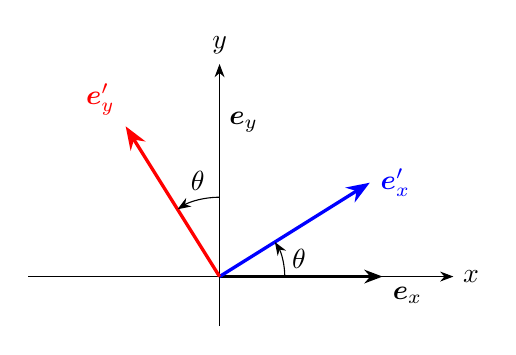
\begin{tikzpicture}[>=Stealth,scale=1.8]
 \def\ang{32}
 \draw[->] (-1.35,0)--(1.65,0) node[right] {$x$};
 \draw[->] (0,-.35)--(0,1.5) node[above] {$y$};
 \draw[->,thick] (0,0)--(1.15,0) node[below right] {$\unit{x}$};
 \draw[->,very thick,blue] (0,0)--(\ang:1.25) node[right] {$\unit{x}'$};
 \draw[->,very thick,red] (0,0)--({90+\ang}:1.25) node[above left] {$\unit{y}'$};
 \draw[->] (.46,0) arc[start angle=0,end angle=\ang,radius=.46]
   node[midway,right] {$\theta$};
 \draw[->] (0,.56) arc[start angle=90,end angle={90+\ang},radius=.56]
   node[midway,above] {$\theta$};
 \node[above right] at (0,.95) {$\unit{y}$};
\end{tikzpicture}
\caption{標準基底を反時計回りに角 $\theta$ だけ回転する}
\end{figure}

回転の一次変換を $R(\theta)$ とすると、
\[
 \begin{pmatrix}\cos\theta\\\sin\theta\end{pmatrix}
 =R(\theta)\begin{pmatrix}1\\0\end{pmatrix},\qquad
 \begin{pmatrix}-\sin\theta\\\cos\theta\end{pmatrix}
 =R(\theta)\begin{pmatrix}0\\1\end{pmatrix}.
\]
これらをまとめると、
\begin{equation}
 \boxed{R(\theta)=
 \begin{pmatrix}
  \cos\theta&-\sin\theta\\
  \sin\theta& \cos\theta
 \end{pmatrix}}
\end{equation}
となる。

次に、ベクトル $\vect{v}$ に角 $\alpha$ と角 $\beta$ の変換を順に
作用させると、
\[
 \vect{v}''=R(\beta)\vect{v}'=R(\beta)R(\alpha)\vect{v}.
\]
図から、これは $\vect{v}$ に角 $\alpha+\beta$ の変換を作用させる
ことと同じなので、
\begin{equation}
 \boxed{R(\alpha+\beta)=R(\beta)R(\alpha)}
\end{equation}
である。

\begin{figure}[htbp]
\centering
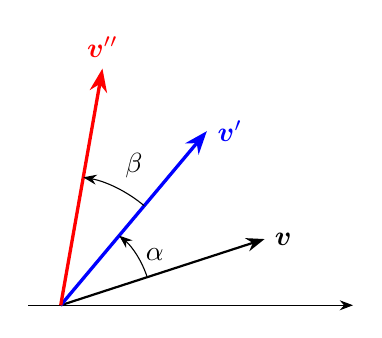
\begin{tikzpicture}[>=Stealth,scale=1.65]
 \draw[->] (-.25,0)--(2.25,0);
 \draw[->,thick] (0,0)--(18:1.65) node[right] {$\vect{v}$};
 \draw[->,very thick,blue] (0,0)--(50:1.75) node[right] {$\vect{v}'$};
 \draw[->,very thick,red] (0,0)--(80:1.85) node[above] {$\vect{v}''$};
 \draw[->] (18:.7) arc[start angle=18,end angle=50,radius=.7]
   node[midway,right] {$\alpha$};
 \draw[->] (50:1.0) arc[start angle=50,end angle=80,radius=1]
   node[midway,above right] {$\beta$};
\end{tikzpicture}
\caption{回転の合成}
\end{figure}

\paragraph{演習}
$R(\alpha+\beta)=R(\alpha)R(\beta)$ から、三角関数の加法定理
\begin{align*}
 \cos(\alpha+\beta)&=\cos\alpha\cos\beta-\sin\alpha\sin\beta,\\
 \sin(\alpha+\beta)&=\sin\alpha\cos\beta+\cos\alpha\sin\beta
\end{align*}
を求めよ。

\subsubsection{基底の変換}

たとえば、3次元の正規直交基底を
\[
 (\unit{1},\unit{2},\unit{3})
 \longrightarrow(\unit{1}',\unit{2}',\unit{3}')
\]
と変換する。このとき、ベクトル $\vect{v}$ の成分はどのように
変換されるだろうか。

ベクトルそのものは基底を変換しても変化しないので、
\begin{equation}
 \vect{v}
 =(\unit{1}\ \unit{2}\ \unit{3})
  \begin{pmatrix}x_1\\x_2\\x_3\end{pmatrix}
 =(\unit{1}'\ \unit{2}'\ \unit{3}')
  \begin{pmatrix}x_1'\\x_2'\\x_3'\end{pmatrix}
\end{equation}
である。ここで、基底の変換を $A$ とすると、
\[
 (\unit{1}'\ \unit{2}'\ \unit{3}')
 =(\unit{1}\ \unit{2}\ \unit{3})A.
\]
したがって
\[
 (\unit{1}'\ \unit{2}'\ \unit{3}')
 \begin{pmatrix}x_1'\\x_2'\\x_3'\end{pmatrix}
 =(\unit{1}\ \unit{2}\ \unit{3})AA^{-1}
 \begin{pmatrix}x_1\\x_2\\x_3\end{pmatrix}
\]
となり、新しい基底でのベクトルの成分は
\begin{equation}
 \boxed{
 \begin{pmatrix}x_1'\\x_2'\\x_3'\end{pmatrix}
 =A^{-1}\begin{pmatrix}x_1\\x_2\\x_3\end{pmatrix}}
\end{equation}
と変換される。

\begin{example}[座標軸の反転]
$y$ 軸を反転した座標系を考える。
\[
 (\unit{x}\ \unit{y})
 =\begin{pmatrix}1&0\\0&1\end{pmatrix}
 \longrightarrow
 \begin{pmatrix}1&0\\0&-1\end{pmatrix}
 =(\unit{x}'\ \unit{y}').
\]

\begin{figure}[htbp]
\centering
\begin{tikzpicture}[>=Stealth]
 \begin{scope}[xshift=-3cm]
  \draw[->] (0,0)--(1.6,0) node[right] {$x$};
  \draw[->] (0,0)--(0,1.4) node[above] {$y$};
 \end{scope}
 \draw[->,thick] (-.8,.7)--(.8,.7) node[midway,above] {$y$軸を反転};
 \begin{scope}[xshift=3cm]
  \draw[->] (0,0)--(1.6,0) node[right] {$x'$};
  \draw[->] (0,1.1)--(0,-1.4) node[below] {$y'$};
 \end{scope}
\end{tikzpicture}
\caption{$y$ 軸を反転した座標系}
\end{figure}

基底の変換行列は
\[
 A=\begin{pmatrix}1&0\\0&-1\end{pmatrix}
\]
である。したがって、位置ベクトルの成分は
\begin{equation}
 \begin{pmatrix}x'\\y'\end{pmatrix}
 =A^{-1}\begin{pmatrix}x\\y\end{pmatrix}
 =\begin{pmatrix}1&0\\0&-1\end{pmatrix}
  \begin{pmatrix}x\\y\end{pmatrix}
\end{equation}
と変換される。
\end{example}

\subsection{固有値・固有ベクトル}

固有値と固有ベクトルは、行列が表す一次変換の本質的な性質を示す
指標である。

\subsubsection{定義と求め方}

$n$ 次正方行列 $A$ に対し、零ベクトルでないベクトル $\vect{v}$ と
スカラー $\lambda$ が
\begin{equation}
 A\vect{v}=\lambda\vect{v},\qquad \vect{v}\ne\vect{0}
\end{equation}
を満たすとき、$\lambda$ を $A$ の\textbf{固有値}、
$\vect{v}$ を固有値 $\lambda$ に属する $A$ の
\textbf{固有ベクトル}という。固有ベクトルは、一次変換 $A$ によって
向きが変わらず、$\lambda$ 倍されるベクトルである。

上の式は
\[
 (A-\lambda I)\vect{v}=\vect{0}
\]
と書ける。この同次連立方程式が $\vect{v}\ne\vect{0}$ という
非自明解をもつためには、係数行列 $A-\lambda I$ が正則であっては
ならない。したがって
\begin{equation}
 \boxed{\det(A-\lambda I)=0}
\end{equation}
が必要である。この $\lambda$ の方程式を $A$ の
\textbf{固有方程式}という。固有方程式を解いて固有値を求め、
各固有値について $(A-\lambda I)\vect{v}=\vect{0}$ を解けば、
固有ベクトルが得られる。

\begin{example}[固有値と固有ベクトル]
\[
 A=\begin{pmatrix}2&1\\3&4\end{pmatrix}
\]
の固有値と固有ベクトルを求める。固有方程式は
\begin{align*}
 \det(A-\lambda I)
 &=\begin{vmatrix}2-\lambda&1\\3&4-\lambda\end{vmatrix}\\
 &=\lambda^2-6\lambda+5
  =(\lambda-1)(\lambda-5)=0
\end{align*}
であるから、固有値は $\lambda=1,5$ である。

$\lambda=1$ のとき、
\[
 (A-I)\vect{v}
 =\begin{pmatrix}1&1\\3&3\end{pmatrix}
  \begin{pmatrix}x\\y\end{pmatrix}
 =\begin{pmatrix}0\\0\end{pmatrix}
\]
より $x+y=0$ なので、固有ベクトルは
\[
 \vect{v}=c\begin{pmatrix}1\\-1\end{pmatrix}\qquad(c\ne0)
\]
である。同様に、$\lambda=5$ のとき
\[
 (A-5I)\vect{v}
 =\begin{pmatrix}-3&1\\3&-1\end{pmatrix}
  \begin{pmatrix}x\\y\end{pmatrix}
 =\begin{pmatrix}0\\0\end{pmatrix}
\]
より $y=3x$ なので、固有ベクトルは
\[
 \vect{v}=c\begin{pmatrix}1\\3\end{pmatrix}\qquad(c\ne0)
\]
である。
\end{example}

\paragraph{演習}
\[
 A=\begin{pmatrix}3&1\\1&3\end{pmatrix}
\]
の固有値と固有ベクトルを求めよ。

\subsubsection{固有値・固有ベクトルの性質}

\paragraph{異なる固有値に属する固有ベクトル}
異なる固有値に属する固有ベクトルは線形独立である。
実際、$\lambda_1\ne\lambda_2$ に属する固有ベクトルを
$\vect{v}_1,\vect{v}_2$ とし、
\[
 x_1\vect{v}_1+x_2\vect{v}_2=\vect{0}
\]
とする。両辺に $A$ を作用させた式から、元の式を
$\lambda_1$ 倍した式を引くと、
\[
 x_2(\lambda_2-\lambda_1)\vect{v}_2=\vect{0}
\]
となる。$\lambda_2-\lambda_1\ne0$ かつ $\vect{v}_2\ne\vect{0}$
なので $x_2=0$ であり、元の式から $x_1=0$ も従う。
よって $\vect{v}_1,\vect{v}_2$ は線形独立である。
一般に、互いに異なる固有値に属する固有ベクトルの組は線形独立である。

\paragraph{行列式とトレース}
2次正方行列
\[
 A=\begin{pmatrix}a_{11}&a_{12}\\a_{21}&a_{22}\end{pmatrix}
\]
の固有値を $\lambda_1,\lambda_2$ とする。固有多項式は
\begin{align*}
 \det(A-\lambda I)
 &=\lambda^2-(a_{11}+a_{22})\lambda
   +(a_{11}a_{22}-a_{12}a_{21})\\
 &=(\lambda-\lambda_1)(\lambda-\lambda_2)
\end{align*}
である。係数を比較すると
\begin{equation}
 \boxed{\det A=\lambda_1\lambda_2,\qquad
        \operatorname{tr}A=\lambda_1+\lambda_2}
\end{equation}
を得る。一般の $n$ 次正方行列でも、重複度を込めて
\[
 \det A=\prod_{i=1}^n\lambda_i,\qquad
 \operatorname{tr}A=\sum_{i=1}^n\lambda_i
\]
が成り立つ。

\subsubsection{行列の対角化}

$n$ 次正方行列 $A$ が線形独立な固有ベクトル
$\vect{v}_1,\ldots,\vect{v}_n$ をもち、対応する固有値を
$\lambda_1,\ldots,\lambda_n$ とする。固有ベクトルを列に並べた行列
\[
 P=(\vect{v}_1\ \vect{v}_2\ \cdots\ \vect{v}_n)
\]
は正則であり、
\begin{align*}
 AP
 &=(A\vect{v}_1\ A\vect{v}_2\ \cdots\ A\vect{v}_n)\\
 &=(\lambda_1\vect{v}_1\ \lambda_2\vect{v}_2\
    \cdots\ \lambda_n\vect{v}_n)\\
 &=P\begin{pmatrix}
 \lambda_1&&0\\
 &\ddots&\\
 0&&\lambda_n
 \end{pmatrix}
\end{align*}
となる。したがって
\begin{equation}
 \boxed{D=P^{-1}AP
 =\begin{pmatrix}
 \lambda_1&&0\\
 &\ddots&\\
 0&&\lambda_n
 \end{pmatrix}}
\end{equation}
である。このように、正則行列 $P$ によって $P^{-1}AP$ を対角行列に
することを、$A$ を\textbf{対角化する}という。なお、すべての行列が
対角化できるわけではなく、$n$ 個の線形独立な固有ベクトルをもつことが
対角化可能であるための必要十分条件である。

対角化できる行列では $A=PDP^{-1}$ なので、
\begin{equation}
 \boxed{A^m=PD^mP^{-1}}
\end{equation}
となり、高いべきも容易に計算できる。

\begin{example}[対角化による行列のべき]
\[
 A=\begin{pmatrix}2&1\\3&4\end{pmatrix}
\]
について、前の例で求めた固有ベクトルを用いると
\[
 P=\begin{pmatrix}1&1\\-1&3\end{pmatrix},\qquad
 D=\begin{pmatrix}1&0\\0&5\end{pmatrix},\qquad
 P^{-1}=\frac14\begin{pmatrix}3&-1\\1&1\end{pmatrix}.
\]
したがって、非負整数 $m$ に対して
\begin{align}
 A^m
 &=P\begin{pmatrix}1&0\\0&5^m\end{pmatrix}P^{-1}\notag\\
 &=\frac14
 \begin{pmatrix}
 3+5^m&-1+5^m\\
 -3+3\cdot5^m&1+3\cdot5^m
 \end{pmatrix}.
\end{align}
\end{example}

\subsubsection{対称行列の固有値・固有ベクトル}

実対称行列 $A=A^{\mathsf T}$ の固有値はすべて実数であり、異なる
固有値に属する固有ベクトルは互いに直交する。さらに、固有ベクトルを
適切に選ぶことで正規直交基底を作ることができる。したがって、ある
直交行列 $U$ を用いて
\begin{equation}
 \boxed{U^{\mathsf T}AU=D}
\end{equation}
と対角化できる。これは実対称行列の\textbf{スペクトル定理}である。

\begin{example}[対称行列の直交対角化]
\[
 A=\begin{pmatrix}7&2\\2&4\end{pmatrix}
\]
の固有値は $\lambda_1=8,\lambda_2=3$ であり、対応する単位固有ベクトル
として
\[
 \vect{u}_1=\frac1{\sqrt5}\begin{pmatrix}2\\1\end{pmatrix},
 \qquad
 \vect{u}_2=\frac1{\sqrt5}\begin{pmatrix}-1\\2\end{pmatrix}
\]
を選べる。これらは
\[
 \vect{u}_1\mathbin{\boldsymbol{\cdot}}\vect{u}_2=0,\qquad
 \lVert\vect{u}_1\rVert=\lVert\vect{u}_2\rVert=1
\]
を満たす。よって
\[
 U=(\vect{u}_1\ \vect{u}_2)
 =\frac1{\sqrt5}\begin{pmatrix}2&-1\\1&2\end{pmatrix}
\]
は直交行列であり、$U^{-1}=U^{\mathsf T}$ である。実際、
\[
 U^{\mathsf T}AU=\begin{pmatrix}8&0\\0&3\end{pmatrix}.
\]
\end{example}

\subsubsection{2次曲線への応用}

交差項を含む2次曲線
\begin{equation}
 5x^2+2\sqrt3xy+7y^2=4
\end{equation}
を考える。$\vect{x}=(x,y)^{\mathsf T}$ とおくと、
\[
 \vect{x}^{\mathsf T}A\vect{x}=4,\qquad
 A=\begin{pmatrix}5&\sqrt3\\\sqrt3&7\end{pmatrix}
\]
と表せる。$A$ の固有値は $4,8$ であり、対応する単位固有ベクトルを
\[
 \vect{u}_1=\frac12\begin{pmatrix}\sqrt3\\-1\end{pmatrix},
 \qquad
 \vect{u}_2=\frac12\begin{pmatrix}1\\\sqrt3\end{pmatrix}
\]
と選ぶと、
\[
 U=(\vect{u}_1\ \vect{u}_2)
 =\frac12\begin{pmatrix}\sqrt3&1\\-1&\sqrt3\end{pmatrix},
 \qquad
 U^{\mathsf T}AU=\begin{pmatrix}4&0\\0&8\end{pmatrix}=D.
\]
$U$ は角 $-\pi/6$ の回転行列である。座標変換
\[
 \vect{x}=U\vect{x}',\qquad
 \vect{x}'=\begin{pmatrix}x'\\y'\end{pmatrix}
\]
を行うと、
\begin{align*}
 \vect{x}^{\mathsf T}A\vect{x}
 &=(U\vect{x}')^{\mathsf T}A(U\vect{x}')\\
 &=\vect{x}'^{\mathsf T}U^{\mathsf T}AU\vect{x}'
 =\vect{x}'^{\mathsf T}D\vect{x}'
\end{align*}
なので、曲線の方程式は
\[
 4{x'}^2+8{y'}^2=4,
 \qquad\text{すなわち}\qquad
 \boxed{{x'}^2+\frac{{y'}^2}{(1/\sqrt2)^2}=1}
\]
となる。したがって、もとの曲線は主軸の方向が座標軸から
$-\pi/6$ だけ回転した楕円である。

\begin{center}
\centering
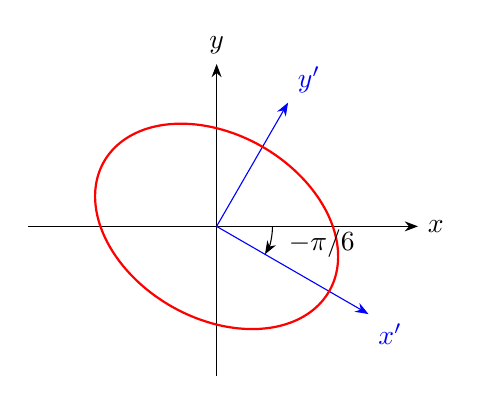
\begin{tikzpicture}[>=Stealth,scale=1.65]
 \def\ang{-30}
 \draw[->] (-1.45,0)--(1.55,0) node[right] {$x$};
 \draw[->] (0,-1.15)--(0,1.25) node[above] {$y$};
 \draw[->,blue] (0,0)--(\ang:1.35) node[below right] {$x'$};
 \draw[->,blue] (0,0)--({90+\ang}:1.1) node[above right] {$y'$};
 \draw[rotate=\ang,thick,red]
   plot[domain=0:360,samples=100,smooth]
   ({cos(\x)},{sin(\x)/sqrt(2)});
 \draw[->] (.43,0) arc[start angle=0,end angle=\ang,radius=.43];
 \node[right] at (.48,-.13) {$-\pi/6$};
\end{tikzpicture}

\smallskip
\refstepcounter{figure}\small 図\thefigure\quad
固有ベクトルの方向を主軸とする楕円
\end{center}


\section{微分学}

\subsection{微分}

\subsubsection{微分係数と導関数}

関数 $y=f(x)$ において、$x$ を $\Delta x$ だけ変化させたときの
$y$ の変化量は $\Delta y=f(x+\Delta x)-f(x)$ である。その比
\[
 \frac{\Delta y}{\Delta x}
 =\frac{f(x+\Delta x)-f(x)}{\Delta x}
\]
を平均変化率という。$\Delta x\to0$ の極限が存在するとき、
\begin{equation}
 \boxed{f'(x)=\lim_{\Delta x\to0}
 \frac{f(x+\Delta x)-f(x)}{\Delta x}}
\end{equation}
を $f$ の\textbf{導関数}という。$x=a$ における値 $f'(a)$ は
微分係数であり、曲線 $y=f(x)$ の点 $(a,f(a))$ における接線の傾きである。

\begin{center}
\begin{tikzpicture}[>=Stealth,scale=1.15]
 \draw[->] (-.4,0)--(5.2,0) node[right] {$x$};
 \draw[->] (0,-.3)--(0,3.5) node[above] {$y$};
 \draw[thick,domain=-.1:4.5,samples=80,smooth]
   plot(\x,{.16*(\x-1.2)^2+.5});
 \coordinate (P) at (2,{.16*(2-1.2)^2+.5});
 \coordinate (Q) at (4,{.16*(4-1.2)^2+.5});
 \fill (P) circle (1.5pt) node[below left] {$P$};
 \fill (Q) circle (1.5pt) node[above left] {$Q$};
 \draw[dashed] (P)--(2,0) node[below] {$x$};
 \draw[dashed] (Q)--(4,0) node[below] {$x+\Delta x$};
 \draw[blue,thick] ($(P)!-.35!(Q)$)--($(P)!1.25!(Q)$)
   node[right] {割線};
 \draw[red,thick] (.5,.22)--(3.8,1.07) node[right] {接線};
\end{tikzpicture}

\small 図\thefigure\quad 割線は $\Delta x\to0$ で接線に近づく
\end{center}

高階導関数は
\[
 f''(x)=\frac{d^2f}{dx^2},\qquad
 f^{(n)}(x)=\frac{d^nf}{dx^n}
\]
と表す。また $x=a$ における値は
$f^{(n)}(a)=\left.\dfrac{d^nf}{dx^n}\right|_{x=a}$ と書く。

\subsubsection{定義から導く基本公式}

\paragraph{べき関数}
二項定理を用いると
\begin{align*}
 \frac{(x+\Delta x)^n-x^n}{\Delta x}
 &=nx^{n-1}+\binom n2x^{n-2}\Delta x+\cdots+(\Delta x)^{n-1}.
\end{align*}
したがって
\begin{equation}
 \boxed{\frac{d}{dx}x^n=nx^{n-1}}
\end{equation}
である。

\paragraph{指数関数}
自然対数の底 $e$ は
\[
 \lim_{h\to0}\frac{e^h-1}{h}=1
\]
を満たすので、
\[
 \frac{d}{dx}e^x
 =e^x\lim_{h\to0}\frac{e^h-1}{h}=e^x.
\]

\paragraph{三角関数}
加法定理から
\begin{align*}
 \frac{\sin(x+h)-\sin x}{h}
 &=\sin x\,\frac{\cos h-1}{h}
   +\cos x\,\frac{\sin h}{h}.
\end{align*}
ここで
\[
 \lim_{h\to0}\frac{\sin h}{h}=1,\qquad
 \lim_{h\to0}\frac{\cos h-1}{h}=0
\]
であるから、$(\sin x)'=\cos x$ を得る。

最初の極限は単位円上の面積比較から示せる。$0<h<\pi/2$ について
\[
 \frac12\sin h<\frac12h<\frac12\tan h
\]
なので、$\cos h<\sin h/h<1$ である。$h\to0$ として挟み撃ちの
原理を用いればよい。また、余弦の加法定理を用いると
\begin{align*}
 \frac{\cos(x+h)-\cos x}{h}
 &=\cos x\,\frac{\cos h-1}{h}
   -\sin x\,\frac{\sin h}{h}\\
 &\longrightarrow-\sin x
\end{align*}
なので、$(\cos x)'=-\sin x$ である。

\begin{center}
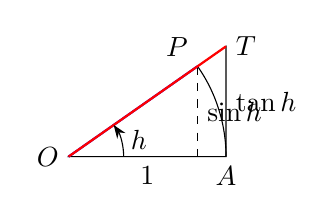
\begin{tikzpicture}[>=Stealth,scale=2]
 \coordinate (O) at (0,0);
 \coordinate (A) at (1,0);
 \coordinate (B) at ({cos(35)},{sin(35)});
 \coordinate (T) at (1,{tan(35)});
 \draw (O)--(A) arc[start angle=0,end angle=35,radius=1]--cycle;
 \draw (A)--(T)--(O);
 \draw[dashed] (B)--({cos(35)},0);
 \draw[thick,blue] (O)--(B);
 \draw[thick,red] (O)--(T);
 \draw[->] (.35,0) arc[start angle=0,end angle=35,radius=.35]
   node[midway,right] {$h$};
 \node[below] at (A) {$A$};
 \node[above left] at (B) {$P$};
 \node[right] at (T) {$T$};
 \node[left] at (O) {$O$};
 \node[below] at (.5,0) {$1$};
 \node[right] at ({cos(35)},{sin(35)/2}) {$\sin h$};
 \node[right] at (1,{tan(35)/2}) {$\tan h$};
\end{tikzpicture}

\small 単位円上の三角形と扇形の面積比較
\end{center}

\paragraph{対数関数}
$x>0$ とし、$h/x=1/n$ とおくと
\begin{align*}
 \frac{\log(x+h)-\log x}{h}
 &=\frac1x\frac{x}{h}\log\left(1+\frac hx\right)\\
 &=\frac1x\log\left(1+\frac1n\right)^n\longrightarrow\frac1x.
\end{align*}
したがって $(\log x)'=1/x$ である。ここでは $\log$ は自然対数を表す。

\subsubsection{微分法則}

微分可能な関数 $f,g$ について
\begin{align}
 (f+g)'&=f'+g',\\
 (fg)'&=f'g+fg',\\
 \left(\frac fg\right)'&=\frac{f'g-fg'}{g^2}\qquad(g\ne0)
\end{align}
が成り立つ。積の微分は、途中に $f(x)g(x+h)$ を挿入して
\begin{align*}
 \frac{f(x+h)g(x+h)-f(x)g(x)}h
 &=\frac{f(x+h)-f(x)}h\,g(x+h)\\
 &\quad+f(x)\frac{g(x+h)-g(x)}h
\end{align*}
と分け、$h\to0$ とすれば得られる。商の微分は
$f/g=f\cdot g^{-1}$ とみなし、
\[
 (g^{-1})'=-\frac{g'}{g^2}
\]
を積の微分と組み合わせれば導ける。

合成関数 $f(g(x))$ について、$\Delta g=g(x+\Delta x)-g(x)$ とおくと
\[
 \frac{f(g+\Delta g)-f(g)}{\Delta x}
 =\frac{f(g+\Delta g)-f(g)}{\Delta g}\frac{\Delta g}{\Delta x}.
\]
極限を取ることにより、\textbf{連鎖律}
\begin{equation}
 \boxed{\frac{d}{dx}f(g(x))=f'(g(x))g'(x)}
\end{equation}
を得る。たとえば
\[
 \frac{d}{dx}\sqrt{1+x^2}=\frac{x}{\sqrt{1+x^2}},\qquad
 \frac{d}{dx}\tan x=\frac1{\cos^2x}.
\]

\subsubsection{停留点・極値・変曲点}

$f'(a)=0$ となる点 $x=a$ を\textbf{停留点}という。停留点の前後で
$f'$ が正から負へ変われば極大、負から正へ変われば極小である。
$f''(a)<0$ なら極大、$f''(a)>0$ なら極小と判定できるが、
$f''(a)=0$ の場合は高階導関数や $f'$ の符号を調べる必要がある。
また、曲線の凹凸が変わる点を\textbf{変曲点}という。$f''(a)=0$ は
候補を与えるだけで、前後で $f''$ の符号が変わることを確認する。

\begin{center}
\begin{tikzpicture}[>=Stealth,scale=.9]
 \draw[->] (-4.6,0)--(4.8,0) node[right] {$x$};
 \draw[->] (0,-2.2)--(0,2.8) node[above] {$y$};
 \draw[thick,smooth] plot coordinates {
 (-4,-1)(-3.2,1.4)(-2.5,2)(-1.8,1.2)(-.8,.3)
 (0,-.2)(.8,-.25)(1.8,-.8)(2.7,-1.6)(3.5,-.8)(4.3,1.3)};
 \foreach \x/\y/\lab in {-2.5/2/A,.8/-.25/C,2.7/-1.6/E}
   {\fill (\x,\y) circle (1.7pt); \draw[dashed] (\x,\y)--(\x,0)
    node[above right] {$x_{\lab}$};}
 \foreach \x/\y/\lab in {-1.55/.92/B,1.75/-.76/D}
   {\fill (\x,\y) circle (1.4pt); \draw[densely dashed,gray] (\x,\y)--(\x,0)
    node[below] {$x_{\lab}$};}
\end{tikzpicture}

\small 極大点 $x_A$、極小点 $x_E$、停留点 $x_C$ と
変曲点 $x_B,x_D$
\end{center}

\paragraph{演習}
\[
 f(x)=\frac15x^5-\frac34x^4+\frac13x^3+\frac32x^2-2x
\]
の増減、極値および変曲点を調べよ。

\paragraph{解答}
\begin{align*}
 f'(x)
 &=x^4-3x^3+x^2+3x-2\\
 &=(x+1)(x-1)^2(x-2)
\end{align*}
である。よって
\[
\begin{array}{c|ccccccc}
x&(-\infty,-1)&-1&(-1,1)&1&(1,2)&2&(2,\infty)\\ \hline
f'(x)&+&0&-&0&-&0&+
\end{array}
\]
となる。したがって $x=-1$ で極大、$x=2$ で極小となり、
$x=1$ は停留点だが極値ではない。関数値は
\[
 f(-1)=\frac{133}{60},\qquad
 f(1)=-\frac{43}{60},\qquad
 f(2)=-\frac{14}{15}
\]
である。

また
\begin{align*}
 f''(x)
 &=4x^3-9x^2+2x+3\\
 &=(x-1)(4x^2-5x-3)\\
 &=4(x-1)
 \left(x-\frac{5-\sqrt{73}}8\right)
 \left(x-\frac{5+\sqrt{73}}8\right).
\end{align*}
各零点の前後で $f''$ の符号が変わるので、変曲点の $x$ 座標は
\[
 \boxed{x=\frac{5-\sqrt{73}}8,\quad1,\quad
        \frac{5+\sqrt{73}}8}
\]
である。

\subsection{Taylor展開と数値微分}

\subsubsection{Taylor展開}

$f$ が $x=a$ の近傍で十分な回数だけ微分可能であるとする。
\[
 f(x)=C_0+C_1(x-a)+C_2(x-a)^2+\cdots
\]
とおき、両辺を繰り返し微分して $x=a$ を代入すると
$C_n=f^{(n)}(a)/n!$ を得る。したがって
\begin{equation}
 \boxed{f(x)=\sum_{n=0}^{\infty}
 \frac{f^{(n)}(a)}{n!}(x-a)^n}
\end{equation}
を $a$ のまわりの\textbf{Taylor展開}という。有限次数で打ち切るときは
\[
 f(x)=\sum_{k=0}^{n}\frac{f^{(k)}(a)}{k!}(x-a)^k+R_n(x)
\]
と書き、$R_n$ を剰余項という。Taylorの定理によれば、適切な
$\xi$ が $a$ と $x$ の間に存在して
\[
 R_n(x)=\frac{f^{(n+1)}(\xi)}{(n+1)!}(x-a)^{n+1}
\]
と表せる。

$a=0$ の場合を\textbf{Maclaurin展開}という。代表例は
\begin{align}
 e^x&=1+x+\frac{x^2}{2!}+\frac{x^3}{3!}+\cdots,\\
 \sin x&=x-\frac{x^3}{3!}+\frac{x^5}{5!}-\cdots,\\
 \cos x&=1-\frac{x^2}{2!}+\frac{x^4}{4!}-\cdots,\\
 (1+x)^\alpha
 &=1+\alpha x+\frac{\alpha(\alpha-1)}{2!}x^2+\cdots
 \qquad(|x|<1)
\end{align}
である。たとえば
\[
 \sqrt{1+x}=1+\frac12x-\frac18x^2+O(x^3),
\qquad
 \frac1{1+x}=1-x+x^2+O(x^3).
\]
ここで $O(x^m)$ は、$x\to0$ のとき絶対値が定数倍の $|x|^m$
以下で抑えられる項を表す。

\paragraph{係数計算の例}
$f(x)=\sin x$ では
\[
 f(0)=0,\quad f'(0)=1,\quad f''(0)=0,\quad
 f^{(3)}(0)=-1,\quad f^{(4)}(0)=0
\]
なので、3次までなら
\[
 \sin x=x-\frac{x^3}{3!}+O(x^5).
\]
$f(x)=\sqrt{1+x}$ では
\[
 f(0)=1,\qquad f'(x)=\frac12(1+x)^{-1/2},\qquad
 f''(x)=-\frac14(1+x)^{-3/2}
\]
より
\[
 f'(0)=\frac12,\qquad f''(0)=-\frac14,
\]
したがって
\[
 \sqrt{1+x}
 =1+\frac12x+\frac{f''(0)}{2!}x^2+O(x^3)
 =1+\frac12x-\frac18x^2+O(x^3)
\]
となる。

\subsubsection{数値微分}

関数値が離散的な点でしか得られない場合、導関数を差分で近似する。
Taylor展開
\begin{align*}
 f(x+h)&=f(x)+f'(x)h+\frac12f''(x)h^2+O(h^3),\\
 f(x-h)&=f(x)-f'(x)h+\frac12f''(x)h^2+O(h^3)
\end{align*}
から、前進差分と後退差分
\begin{align}
 f'(x)&=\frac{f(x+h)-f(x)}h+O(h),\\
 f'(x)&=\frac{f(x)-f(x-h)}h+O(h)
\end{align}
を得る。両者を平均すると1次の誤差が打ち消され、
\begin{equation}
 \boxed{f'(x)=\frac{f(x+h)-f(x-h)}{2h}+O(h^2)}
\end{equation}
となる。これを\textbf{中心差分}という。

\begin{center}
\begin{tikzpicture}[>=Stealth,scale=1.1]
 \draw[->] (-.4,0)--(5,0) node[right] {$x$};
 \draw[->] (0,-.2)--(0,3.5) node[above] {$y$};
 \draw[thick,domain=.4:4.5,samples=70,smooth]
   plot(\x,{.18*(\x-1.6)^2+.55});
 \foreach \x/\lab in {1.5/{x-h},2.5/x,3.5/{x+h}}
  {\draw[dashed] (\x,0)--(\x,{.18*(\x-1.6)^2+.55});
   \node[below] at (\x,0) {$\lab$};}
 \draw[blue] (2.5,.45)--(4.5,1.8) node[right] {前進};
 \draw[red] (.5,.45)--(2.5,.72) node[left] {後退};
 \draw[green!60!black,thick] (1.1,.2)--(4,1.42) node[right] {中心};
\end{tikzpicture}

\small 前進差分・後退差分・中心差分による傾きの近似
\end{center}

2階微分は二つのTaylor展開を加えることで
\begin{align*}
 f(x+h)+f(x-h)
 &=2f(x)+f''(x)h^2\\
 &\quad+\frac1{12}f^{(4)}(x)h^4+O(h^6)
\end{align*}
となるため、
\begin{equation}
 \boxed{f''(x)=\frac{f(x+h)-2f(x)+f(x-h)}{h^2}+O(h^2)}
\end{equation}
と近似できる。$h$ を小さくすれば打切り誤差は減少するが、極端に
小さくすると浮動小数点の丸め誤差や桁落ちが増えるため、実計算では
両者の釣合いを考える必要がある。

\subsection{多変数関数の微分}

\subsubsection{偏微分}

2変数関数 $z=f(x,y)$ に対し、一方の変数を固定して他方だけを
変化させた微分を\textbf{偏微分}という。
\begin{align}
 f_x(x,y)&=\lim_{h\to0}\frac{f(x+h,y)-f(x,y)}h,\\
 f_y(x,y)&=\lim_{h\to0}\frac{f(x,y+h)-f(x,y)}h.
\end{align}
$f_x=\partial f/\partial x$ などと書く。高階偏導関数は
\[
 f_{xx}=\frac{\partial^2f}{\partial x^2},\quad
 f_{xy}=\frac{\partial^2f}{\partial y\partial x},\quad
 f_{yx}=\frac{\partial^2f}{\partial x\partial y}
\]
と表す。混合偏導関数が近傍で連続なら $f_{xy}=f_{yx}$ である。

\begin{center}
\begin{tikzpicture}[>=Stealth,x={(.85cm,-.35cm)},y={(.85cm,.35cm)},z={(0cm,1cm)}]
 \draw[->] (0,0,0)--(4,0,0) node[below] {$x$};
 \draw[->] (0,0,0)--(0,4,0) node[right] {$y$};
 \draw[->] (0,0,0)--(0,0,3.2) node[above] {$z$};
 \foreach \i in {0,...,4}
  {\draw[gray] plot[domain=0:4,samples=20] (\x,\i,{.08*(\x-2)^2+.08*(\i-2)^2+1});
   \draw[gray] plot[domain=0:4,samples=20] (\i,\x,{.08*(\i-2)^2+.08*(\x-2)^2+1});}
 \fill (2.8,2.3,1.06) circle (1.6pt);
 \draw[blue,thick] (1.5,2.3,.95)--(4,2.3,1.35) node[right] {$x$ 方向};
 \draw[red,thick] (2.8,1,.95)--(2.8,3.8,1.35) node[right] {$y$ 方向};
\end{tikzpicture}

\small 曲面の座標方向に沿った断面の傾きが偏導関数である
\end{center}

\begin{example}
$f(x,y)=2x^2+3xy-y^2+4y^3$ なら
\[
 f_x=4x+3y,\qquad f_y=3x-2y+12y^2
\]
である。
\end{example}

\paragraph{演習}
$f(x,y)=2e^{2x}\sin\sqrt{xy}$ の $f_x,f_y$ を求めよ。ただし $xy>0$
とする。

\paragraph{解答}
$s=\sqrt{xy}$ とおくと
\[
 s_x=\frac{y}{2\sqrt{xy}},\qquad
 s_y=\frac{x}{2\sqrt{xy}}.
\]
積の微分と連鎖律により
\begin{align*}
 f_x
 &=4e^{2x}\sin s+2e^{2x}\cos s\,s_x\\
 &=4e^{2x}\sin\sqrt{xy}
   +e^{2x}\frac{y}{\sqrt{xy}}\cos\sqrt{xy},\\
 f_y
 &=2e^{2x}\cos s\,s_y\\
 &=e^{2x}\frac{x}{\sqrt{xy}}\cos\sqrt{xy}.
\end{align*}

\subsubsection{全微分と連鎖律}

$f(x,t)$ で $x=x(t)$ も $t$ に依存するとき、偏微分
$\partial f/\partial t$ は $x$ を固定した変化率である。一方、
合成関数 $f(x(t),t)$ の微分は
\begin{equation}
 \boxed{\frac{df}{dt}
 =\frac{\partial f}{\partial t}
 +\frac{\partial f}{\partial x}\frac{dx}{dt}}
\end{equation}
となる。一般に $z=f(x_1,\ldots,x_n)$ の全微分は
\[
 dz=\sum_{i=1}^n\frac{\partial f}{\partial x_i}\,dx_i
\]
である。

\begin{example}
$f(x,t)=at^2+btx,\ x(t)=\sin t$ とする。連鎖律により
\[
 \frac{df}{dt}=(2at+bx)+(bt)\cos t
 =2at+b\sin t+bt\cos t.
\]
直接 $f(t)=at^2+bt\sin t$ を微分しても同じ結果を得る。
\end{example}

\subsubsection{勾配と方向微分}

スカラー場 $f(x_1,\ldots,x_n)$ に対し
\begin{equation}
 \boxed{\nabla f
 =\left(\frac{\partial f}{\partial x_1},\ldots,
 \frac{\partial f}{\partial x_n}\right)^{\mathsf T}}
\end{equation}
を $f$ の\textbf{勾配}という。単位ベクトル $\vect{u}$ 方向の
方向微分は
\[
 D_{\vect{u}}f=\nabla f\mathbin{\boldsymbol{\cdot}}\vect{u}
 =\lVert\nabla f\rVert\cos\theta
\]
である。したがって $\nabla f$ は $f$ が最も急に増加する方向を向き、
その大きさは最大変化率である。また等高線・等位面に直交する。

\begin{center}
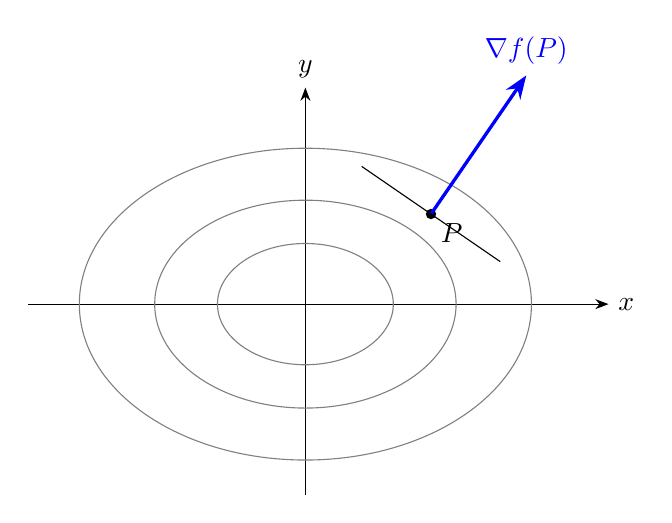
\begin{tikzpicture}[>=Stealth,scale=1.1]
 \draw[->] (-3.2,0)--(3.5,0) node[right] {$x$};
 \draw[->] (0,-2.2)--(0,2.5) node[above] {$y$};
 \foreach \r in {.7,1.2,1.8}{\draw[gray] (0,0) ellipse ({1.45*\r} and \r);}
 \coordinate (P) at (1.45,1.04);
 \fill (P) circle (1.7pt) node[below right] {$P$};
 \draw[->,very thick,blue] (P)--($(P)+(1.1,1.6)$)
   node[above] {$\nabla f(P)$};
 \draw ($(P)+(-.8,.55)$)--($(P)+(.8,-.55)$);
\end{tikzpicture}

\small 勾配は等高線の法線方向を向く
\end{center}

\subsection{微分の応用}

\subsubsection{最小二乗法}

測定点 $(x_i,y_i)\ (i=1,\ldots,N)$ に直線 $y=ax+b$ を当てはめる。
残差 $\varepsilon_i=y_i-(ax_i+b)$ の二乗和
\[
 E(a,b)=\sum_{i=1}^N\{y_i-(ax_i+b)\}^2
\]
を最小にする。停留条件 $E_a=E_b=0$ は
\begin{align*}
 \frac{\partial E}{\partial a}
 &=-2\sum_{i=1}^Nx_i(y_i-ax_i-b)\\
 &=2\left(a\sum x_i^2+b\sum x_i-\sum x_iy_i\right)=0,\\
 \frac{\partial E}{\partial b}
 &=-2\sum_{i=1}^N(y_i-ax_i-b)\\
 &=2\left(a\sum x_i+bN-\sum y_i\right)=0.
\end{align*}
これらを整理すると
\begin{equation}
 \begin{pmatrix}
  \sum x_i^2&\sum x_i\\ \sum x_i&N
 \end{pmatrix}
 \begin{pmatrix}a\\b\end{pmatrix}
 =
 \begin{pmatrix}\sum x_iy_i\\\sum y_i\end{pmatrix}
\end{equation}
となる。これを\textbf{正規方程式}という。分母が零でなければ
\begin{align}
 a&=\frac{N\sum x_iy_i-(\sum x_i)(\sum y_i)}
 {N\sum x_i^2-(\sum x_i)^2},\\
 b&=\frac{(\sum x_i^2)(\sum y_i)-(\sum x_i)(\sum x_iy_i)}
 {N\sum x_i^2-(\sum x_i)^2}.
\end{align}

\begin{center}
\begin{tikzpicture}[>=Stealth,scale=.9]
 \draw[->] (-.2,0)--(6.3,0) node[right] {$x$};
 \draw[->] (0,-.2)--(0,4.5) node[above] {$y$};
 \draw[thick,blue] (.3,.5)--(5.8,3.8) node[right] {$y=ax+b$};
 \foreach \x/\y in {.7/.7,1.3/1.7,2/1.4,2.8/2.5,3.6/2.4,4.3/3.5,5.1/3.2}
  {\fill (\x,\y) circle (1.5pt);\draw[dashed,red] (\x,\y)--(\x,{.6*\x+.32});}
\end{tikzpicture}

\small 測定点と回帰直線。破線は残差を表す
\end{center}

2次関数 $y=ax^2+bx+c$ の場合は
\[
 E(a,b,c)=\sum_{i=1}^N\{y_i-(ax_i^2+bx_i+c)\}^2
\]
の停留条件から
\begin{equation}
 \begin{pmatrix}
 \sum x_i^4&\sum x_i^3&\sum x_i^2\\
 \sum x_i^3&\sum x_i^2&\sum x_i\\
 \sum x_i^2&\sum x_i&N
 \end{pmatrix}
 \begin{pmatrix}a\\b\\c\end{pmatrix}
 =
 \begin{pmatrix}\sum x_i^2y_i\\\sum x_iy_i\\\sum y_i\end{pmatrix}
\end{equation}
を得る。

\subsubsection{画像の勾配とエッジ}

濃淡画像を輝度関数 $\phi(x,y)$ とみなすと、$\nabla\phi$ は輝度が
最も急に増加する方向を示す。したがって $\lVert\nabla\phi\rVert$ が
大きい画素はエッジ候補であり、勾配方向は局所的なエッジの法線方向である。
デジタル画像では中心差分
\[
 \phi_x(i,j)\simeq\frac{\phi(i+1,j)-\phi(i-1,j)}2,\qquad
 \phi_y(i,j)\simeq\frac{\phi(i,j+1)-\phi(i,j-1)}2
\]
などで勾配を近似する。勾配方向の輝度プロファイルを $\psi(t)$ とすると、
滑らかな段差では $|\psi'(t)|$ が極大となる位置、すなわち
$\psi''(t)=0$ 付近をエッジ位置として細かく推定できる。

\begin{center}
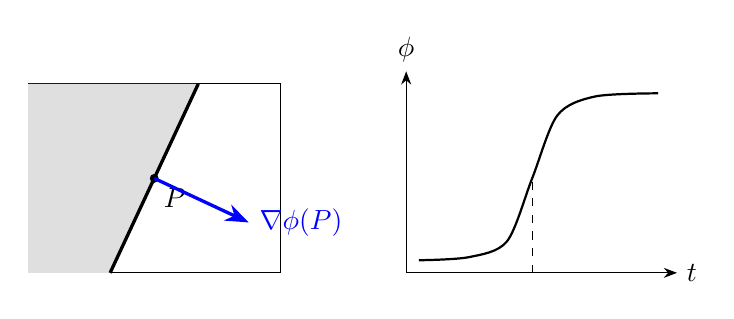
\begin{tikzpicture}[>=Stealth,scale=.8]
 \draw (0,0) rectangle (4,3);
 \fill[gray!25] (0,0)--(0,3)--(2.7,3)--(1.3,0)--cycle;
 \draw[very thick] (1.3,0)--(2.7,3);
 \coordinate (P) at (2,1.5);
 \fill (P) circle (2pt) node[below right] {$P$};
 \draw[->,blue,very thick] (P)--($(P)+(1.5,-.7)$)
   node[right] {$\nabla\phi(P)$};
 \begin{scope}[xshift=6cm]
  \draw[->] (0,0)--(4.3,0) node[right] {$t$};
  \draw[->] (0,0)--(0,3.2) node[above] {$\phi$};
  \draw[thick,smooth] plot coordinates{(.2,.2)(1,.25)(1.6,.5)(2,1.5)
     (2.4,2.5)(3,2.8)(4,2.85)};
  \draw[dashed] (2,0)--(2,1.5);
 \end{scope}
\end{tikzpicture}

\small 画像エッジと勾配方向の輝度プロファイル
\end{center}

\subsubsection{Lagrangeの未定乗数法}

拘束条件 $g(x,y)=0$ のもとで $f(x,y)$ の極値を求める。正則な
拘束曲線上の極値では等高線が接するため $\nabla f=\lambda\nabla g$
となる。Lagrange関数
\[
 L(x,y,\lambda)=f(x,y)-\lambda g(x,y)
\]
を導入すれば、候補点は
\begin{equation}
 \boxed{L_x=L_y=L_\lambda=0}
\end{equation}
を解いて求められる。候補点が最大・最小のどちらかは、関数値の比較や
拘束曲線上での増減により判定する。

\begin{example}
$g(x,y)=y+x^2-2=0$ のもとで $f(x,y)=y-2x$ の極値を求める。
\[
 L=y-2x-\lambda(y+x^2-2)
\]
の停留条件から $(x,y)=(-1,1)$、$f=3$ を得る。拘束条件を代入すると
$f=2-x^2-2x=3-(x+1)^2$ なので、この点で最大値 $3$ をとる。
一方、$|x|\to\infty$ で $f\to-\infty$ となるため、最小値は存在しない。

\begin{center}
\begin{tikzpicture}[>=Stealth,scale=1.05]
 \draw[->] (-3.2,0)--(3.2,0) node[right] {$x$};
 \draw[->] (0,-2.2)--(0,3.1) node[above] {$y$};
 \draw[thick,domain=-2.1:2.1,samples=60,smooth]
   plot(\x,{2-\x*\x}) node[right] {$y=2-x^2$};
 \draw[blue,thick] (-2.4,-1.8)--(.8,4.6)
   node[above right] {$y=2x+3$};
 \fill (-1,1) circle (2pt) node[above left] {$(-1,1)$};
 \draw[dashed] (-1,1)--(-1,0) node[below] {$-1$};
\end{tikzpicture}

\small 目的関数の等高線 $y-2x=3$ が拘束曲線に接する
\end{center}
\end{example}

\begin{example}[楕円に内接する長方形]
楕円 $x^2/a^2+y^2/b^2=1$ に内接する軸平行な長方形の面積は
$S=4xy$ である。第1象限で
\[
 L=4xy-\lambda\left(\frac{x^2}{a^2}+\frac{y^2}{b^2}-1\right)
\]
とおく。停留条件は
\begin{align*}
 L_x&=4y-\frac{2\lambda x}{a^2}=0,\\
 L_y&=4x-\frac{2\lambda y}{b^2}=0,\\
 L_\lambda&=-\left(\frac{x^2}{a^2}+\frac{y^2}{b^2}-1\right)=0.
\end{align*}
最初の二式をそれぞれ $x,y$ 倍すると
\[
 4xy=\frac{2\lambda x^2}{a^2}
     =\frac{2\lambda y^2}{b^2}
\]
なので $x^2/a^2=y^2/b^2$ である。これと拘束条件から
\[
 x=\frac{a}{\sqrt2},\qquad y=\frac{b}{\sqrt2},\qquad
 \boxed{S_{\max}=2ab}
\]
を得る。
\begin{center}
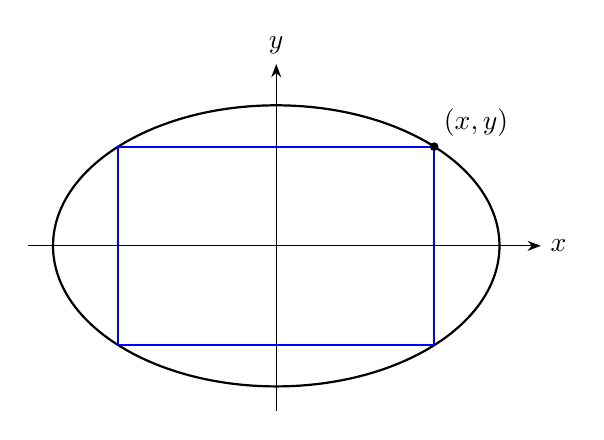
\begin{tikzpicture}[>=Stealth,scale=1.05]
 \draw[->] (-3,0)--(3.2,0) node[right] {$x$};
 \draw[->] (0,-2)--(0,2.2) node[above] {$y$};
 \draw[thick] (0,0) ellipse (2.7 and 1.7);
 \draw[blue,thick] (-1.91,-1.2) rectangle (1.91,1.2);
 \fill (1.91,1.2) circle (1.5pt) node[above right] {$(x,y)$};
\end{tikzpicture}
\end{center}
\end{example}


\end{document}
